\chapter{An Incomplete Theory}
\label{sec:theo}

One of the great questions that humans have always tried to answer is
what are the fundamental building blocks of the universe and what are the rules that govern them?
%Attempts at answering this question have ranged from the
%philosophical approach of \textit{`atomism'} by the ancient Greeks \cite{theo-atomism}
%to the discovery of atomic structure by Ernest Rutherford \cite{theo-rutherford}.
%
The current best answer to this question is the \textit{`Standard Model of Particle Physics'},
a mathematical description of a finite set of fundamental particles and their interactions.
The Standard Model has been found to agree with experimental data at great precision~\cite{theo-ewTests}
and as a result is the foundation of the field of particle physics.
However, it is known that this is not a complete theory and there must be
a deeper underlying theory that lies beyond the Standard Model.

This chapter firstly aims to describe the Standard Model and
possible Beyond Standard Model (BSM) physics in the context of di-$b$-jet searches.
Section~\ref{sec:theo-sm} briefly describes the particles and forces of the Standard Model.
Section~\ref{sec:theo-qcd} describes hadronic jet formation and the production of the dominant Standard Model background to di-$b$-jet searches.
Section~\ref{sec:theo-bsm} will discuss BSM physics;
specifically the problems in the Standard Model that require BSM physics
and proposed BSM models that predict resonances preferentially decaying to one or two $b$-quarks.

\section{The Standard Model}
\label{sec:theo-sm}

The Standard Model is a quantum field theory,
meaning that the theory describes a finite set of particles and their interactions in
terms of a set of fields.
%The end product of the Standard Model is a prediction
%of what will happen when any two particles in nature interact;
%which in the context of a collider experiment means predicting what is the cross-section of any given interaction.

%Section~\ref{sec:theo-sm_particles} contains a description of the particles that make up the Standard Model 
%and Section~\ref{sec:theo-sm_forces} contains a description of the types of interactions between the particles, known as forces.

\subsection{Particles}
\label{sec:theo-sm_particles}

The Standard Model consists of a set of fundamental particles,
where fundamental means that they are not composed of other constituent particles.
Full details of the Standard Model particles are found in~\cite{obj-bjets_PDG}.

\noindent
The particles of the Standard Model form three groups of particles with similar properties.
The particle groups are:

\begin{itemize}[leftmargin=*]
\item\textbf{Quarks:}
  %Quarks are spin-$\frac{1}{2}$ fermions.
  There are 6 different types of quarks, known as flavours, arranged in 3 generations.
  For each quark there is also an anti-quark, which has identical mass and spin, but opposite charge and quantum numbers.  \vspace{1em}
  
\item\textbf{Leptons:}
  %Leptons are fermions that, unlike the quarks, do not interact with the strong force.
  There are 6 different types of leptons,
  arranged into  3 generations, each containing a charge $-1$ particle and a charge 0 neutrino.
  For each lepton there is also an anti-lepton. \vspace{1em}
 
\item\textbf{Bosons:}
  There are a set of integer-spin particles  known as bosons.
  The bosons act as the mediators of the forces that will be described below.  \vspace{1em}
  
\end{itemize}
  
\noindent
Table~\ref{tab:theo-sm_particles} summarises the key properties of the particles in the Standard Model.
%The particles are organised into the particle groups and then into the three generations for the quarks and leptons.

  {\renewcommand{\arraystretch}{1.2}
  \begin{table}[!ht]
  \begin{center}
    \begin{tabular}{|c|c||c|c|c|c|}
      \hline
    Particle Group          & Particle Name   & Symbol        & Charge  &  Spin  &  Mass [GeV]\\
    \hline
    \multirow{6}{*}{Quark}  &Up            &   $u$  &  $+2/3$   &  $1/2$  &  0.002\\
                            &Down          &   $d$  &  $-1/3$   &  $1 / 2$  &  0.005\\
                            \cline{2-6}                                            
                            &Charm         &   $c$  &  $+2/3$   &  $1 / 2$  &  1.3 \\
                            &Strange       &   $s$  &  $-1/3$   &  $1 / 2$  &  0.096 \\
                            \cline{2-6}                                                      
                            &Top           &   $t$  &  $+2/3$   &  $1 / 2$  &  173  \\
                            &Bottom        &   $b$  &  $-1/3$   &  $1 / 2$  &  4.2  \\
    \hline                  
    \multirow{6}{*}{Lepton} &Electron          &   $e$         &  $-1$    &  $1 / 2$   &  \num{5.1e-4}\\
                            &Electron Neutrino &   $\nu_e$     &  0     &  $1 / 2$   &  $< $\num{2e-9}\\
                            \cline{2-6}                                   
                            &Muon              &   $\mu$       &  $-1$    &  $1 / 2$   &  0.11 \\
                            &Muon Neutrino     &   $\nu_{\mu}$  &  0     &  $1 / 2$     &  $<$\num{1.9e-4}\\
                            \cline{2-6}                                      
                            &Tau               &   $\tau$       &  $-1$   &  $1 / 2$   &  1.8\\
                            &Tau Neutrino      &   $\nu_{\tau}$  &  0    &  $1 / 2$     &  $<$\num{1.8e-2}\\
    \hline
    \multirow{5}{*}{Boson}  &Photon           &   $\gamma$    &  0      &  1     &  0 \\
                            &W boson          &   $W^{\pm}$    & $\pm1$  &  1     &  80 \\
                            &Z boson          &   $Z_0$       &  0      &  1     &  91\\
                            &Gluon            &   $g$         &  0      &  1     &  0 \\
                            &Higgs Boson      &   $H$         &  0      &  0     &  125\\
    \hline  
    \end{tabular} 
  \caption[The key properties of the particles in the Standard Model]
          {The key properties of the particles in the Standard Model, organised by particle group and then by generation.
            Values taken from~\cite{obj-bjets_PDG}.}
  \label{tab:theo-sm_particles}
  \end{center}
  \end{table}}

  \newpage
\subsection{Forces}
\label{sec:theo-sm_forces}

The Standard Model combines three key quantum field theories.
%in a $SU(3)~\text{x}~SU(2)~\text{x}~U(1)$ gauge symmetry.
The first is the electro-weak theory~\cite{theo-glashow}
which describes three interactions grouped into two forces: the electro-magnetic and weak forces.
The second is Quantum Chromodynamics (QCD)~\cite{theo-qcd} which describes the strong force.
Finally, the Higgs Mechanism~\cite{theo-higgs,theo-be}~\footnote{Also known as the Englert-Brout-Higgs mechanism.}
describes the origin of mass in the Standard Model \footnote{With the exception of the neutrinos, whose mass is not described by the Standard Model.}.
Each of the forces is discussed below.

\begin{itemize}[leftmargin=*]
\item\textbf{Electro-magnetic (EM) Force:}

  The EM force is an interaction between electrically charged particles and is mediated by the photon.
  The strength of the EM coupling is proportional to the EM coupling constant, $\alpha_{EM}$,
  multiplied by the product of the charges of the two particles, where $\alpha_{EM} \sim$ 1/137.\vspace{1em} %\vspace{1em}

\item\textbf{Weak Force:} \\
  The weak force is composed of the two remaining interactions from electro-weak theory;
  the neutral current interaction and the charged current interaction.
  \begin{itemize}[leftmargin=*]  
  \item The \textit{`neutral current interaction'} is mediated by the $Z_0$ boson, interacts with all fermions,
    and does not allow flavour changing interactions.
  \item The \textit{`charged current interaction'} is mediated by the $W^+$ and $W^-$ bosons,
    has a universal interaction with all fermions,
    and flavour changing interactions are allowed.
    In the quark sector, the charged current interaction
    couples with weak eigenstates of fermions rather than their flavour eigenstates,
    allowing for interactions that change the generation of the quark's flavour.
    The relative amplitudes of each flavour changing interaction is described by the CKM matrix~\cite{theo-ckm};
    the values of this matrix highly suppresses generational changing interactions involving the 3rd generation of quarks.
  %This high supprestion will prove important for identifying the presence of $b$-quarks at the ATLAS detector, which will be discussed in Section~\ref{sec:obj-bjets}.
  \end{itemize}
  At low energies ($Q < m_W$) the weak force is less strong than the EM force due to the large mass of the $W/Z$ boson
  \mbox{($\text{Weak}/\text{EM} \sim 10^{-4}$)} and at larger energies ($Q \geq m_W$)
  the EM force and weak force become comparable in strength.\vspace{1em} %\vspace{0.5em}
  
\item\textbf{Strong Force:}\\
  QCD describes the strong force.
  The strong force is mediated by gluons 
  and interacts with particles that have colour charge; which are quarks and gluons.
  %The fact that the gluon has colour charge means that the gluon is self interacting.
  QCD has 3 colour charges: known as red, green and blue.
  A quark has a colour charge, an anti-quark has an anti colour charge and 
  a gluon has a colour charge and an anti-colour charge, leading to 8 independent colour states of a gluon.
  A colour neutral object can be formed if all three colour charges are present (i.e. in a baryon containing three quarks)
  or if a colour and the corresponding anti-colour is present (i.e. in a meson that contains $q\bar{q}$).
  As QCD describes hadronic jet formation and the largest background in a di-$b$-jet search, QCD is discussed further in Section~\ref{sec:theo-qcd}.\vspace{1em}

\item\textbf{Higgs Mechanism:}\\
  The Higgs mechanism introduces an extra scalar field to the Standard Model
  with a Higgs potential given by the so-called `Mexican-hat potential'.
  This allows for spontaneous symmetry breaking which gives mass to the bosons of the Standard Model.
  In addition, a Yukawa coupling term between the scalar field and the fermions gives rise to the mass of the fermions
  \footnote{With the exception of the neutrinos, whose mass is not described by the Standard Model}.
  A final prediction of the Higgs mechanism is the existence of the Higgs boson.
  The first observation the Higgs boson by the ATLAS~\cite{theo-higgs_atlas} and CMS~\cite{theo-higgs_cms} experiments
  in 2012 confirms the Higgs mechanism, a great triumph of the Standard Model.
\end{itemize}

\section{QCD: Hadronic Jet Formation and Dijet Production}
\label{sec:theo-qcd}

As described above, Quantum Chromodynamics (QCD) is a theory that describes the strong interaction between quarks and gluons.
Section~\ref{sec:theo-qcd_dijet_running} will describe the renormalisation of QCD, which is important for understanding how QCD works.
Then Section~\ref{sec:theo-qcd_jets} will describe the formation of hadronic jets and
Section~\ref{sec:theo-qcd_dijet} will describe the production of dijet events through QCD in $pp$ collisions, which is the dominant background in di-$b$-jet searches;
these two elements of QCD that are critical to the analyses being presented in this thesis.
Quarks and gluons can often fill similar roles in hadronic jet formation and dijet production, hence I will refer to them collectively as `partons' in this section.

\subsection{Renormalisation and the Running of $\alpha_S$}
\label{sec:theo-qcd_dijet_running}

For any calculation in QCD, or indeed any quantum field theory, one must consider the higher-order loop diagrams;
for example a simple gluon propagator has additional first-order loops as shown in Figure~\ref{fig:theo-qcd_gluon}.
The summation over all higher-order loops leads to divergences in calculations of scattering events in QCD.

\begin{figure}[!hbt]
  \begin{center}
    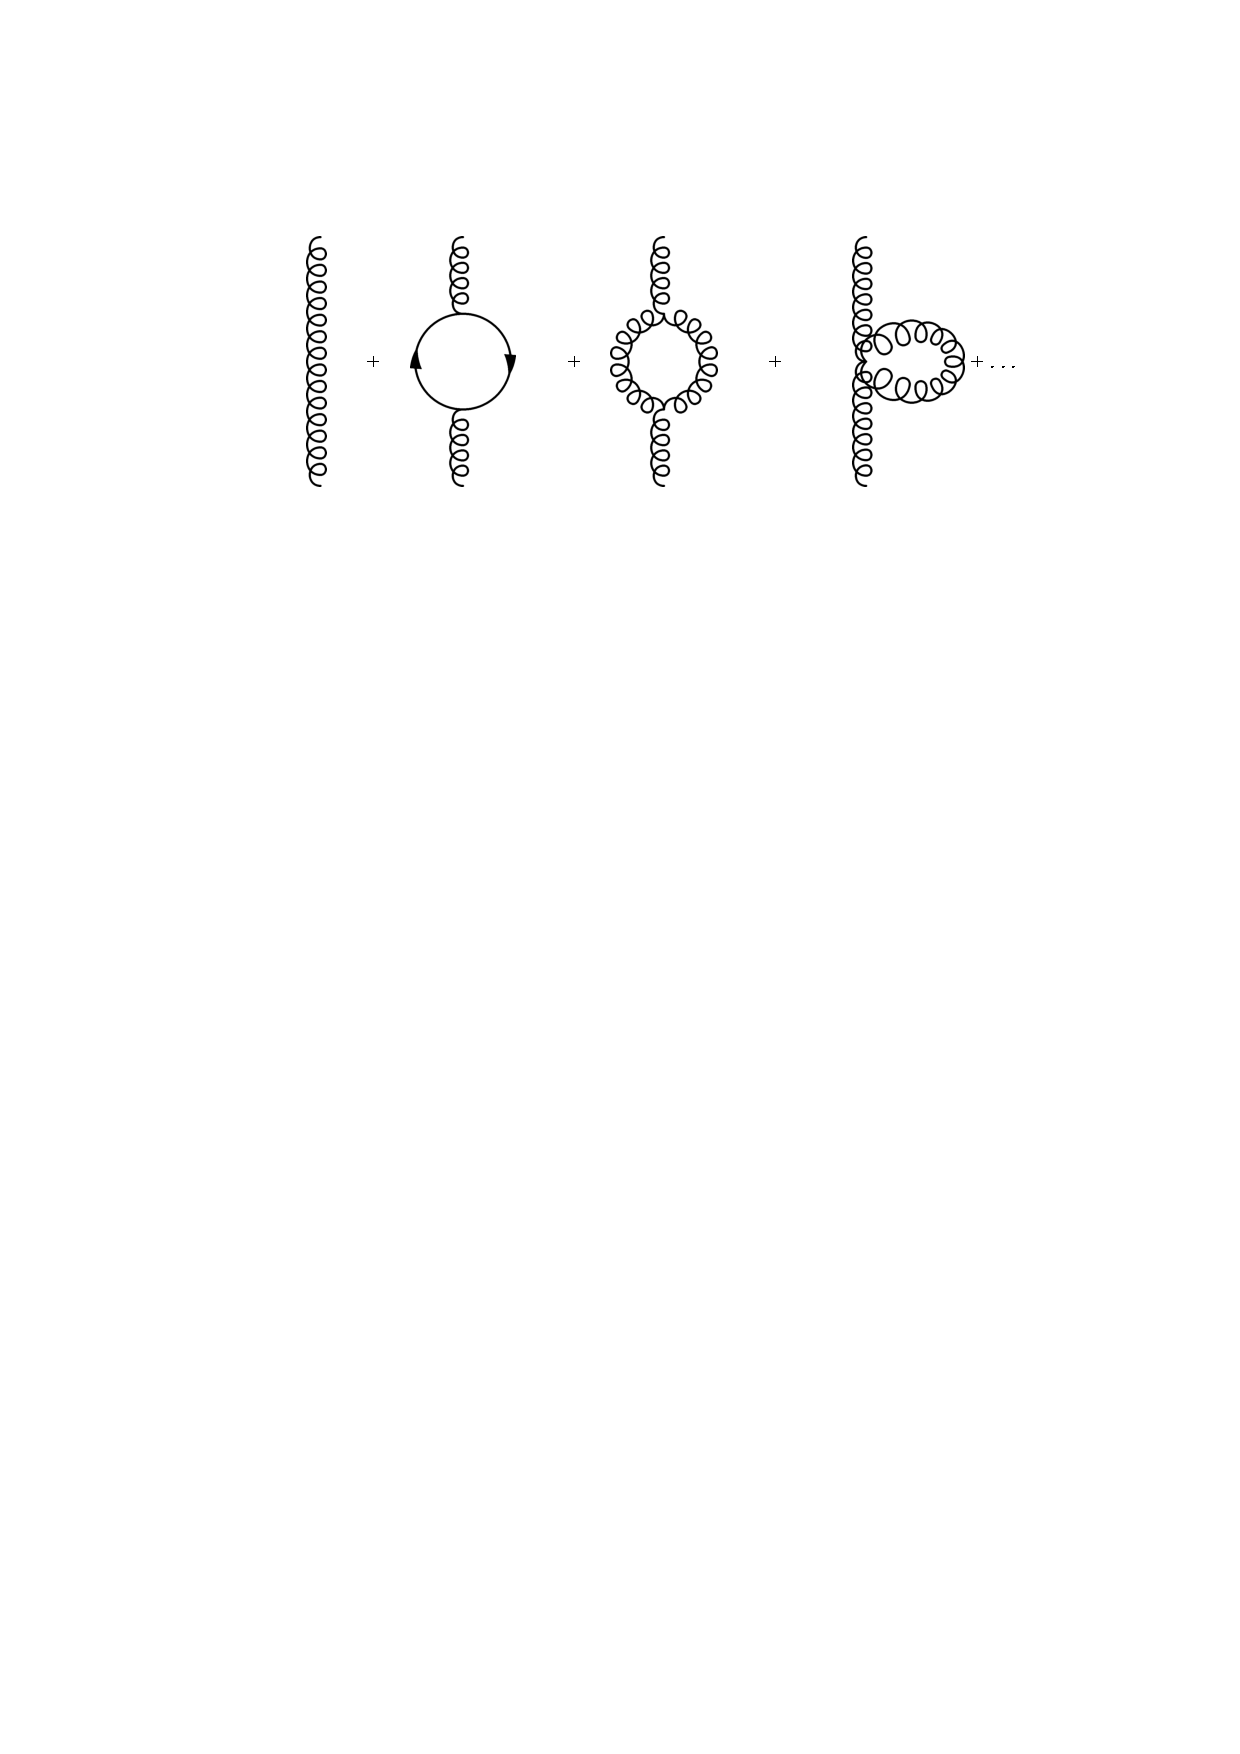
\includegraphics[width=0.5\linewidth, angle=0]{figs/Theory/qcd_gluon_loop.pdf}
  \end{center}
  \vspace{-1em}
  \caption[A schematic showing the gluon propagator with the additional first order loops.]
  {A schematic showing the gluon propagator with the additional first order loops~\cite{det-thesis_kate}.}
  \label{fig:theo-qcd_gluon}
\end{figure}

To avoid these divergences, there is a well accepted mathematical tool, known as renormalisation,
where one effectively re-scales the fields in the Lagrangian~\cite{theo-qcd}.
Renormalisation is done such that the divergences are removed
when performing perturbative calculations of QCD.
This leads to a dependence of the strong coupling constant, $\alpha_S$, on the renormalisation scaled used, $\mu_R$,
an effect known as the running of $\alpha_S$.
To get an effective strength of the strong interaction in any given process,
the value of $\mu_R$ is set as the scale of the momentum transfer, $Q$, of the process.
%%which is the natural choice for the process.
%$\alpha_S($\mu_R \sim Q^{2}$).
The running of $\alpha_{S}$ can be measured through experimental observation;
Figure~\ref{fig:theo-qcd_running} shows the measured values of $\alpha_S$
as a function of the energy scale, $Q$, in a range of experiments.

\begin{figure}[!hbt]
  \begin{center}
    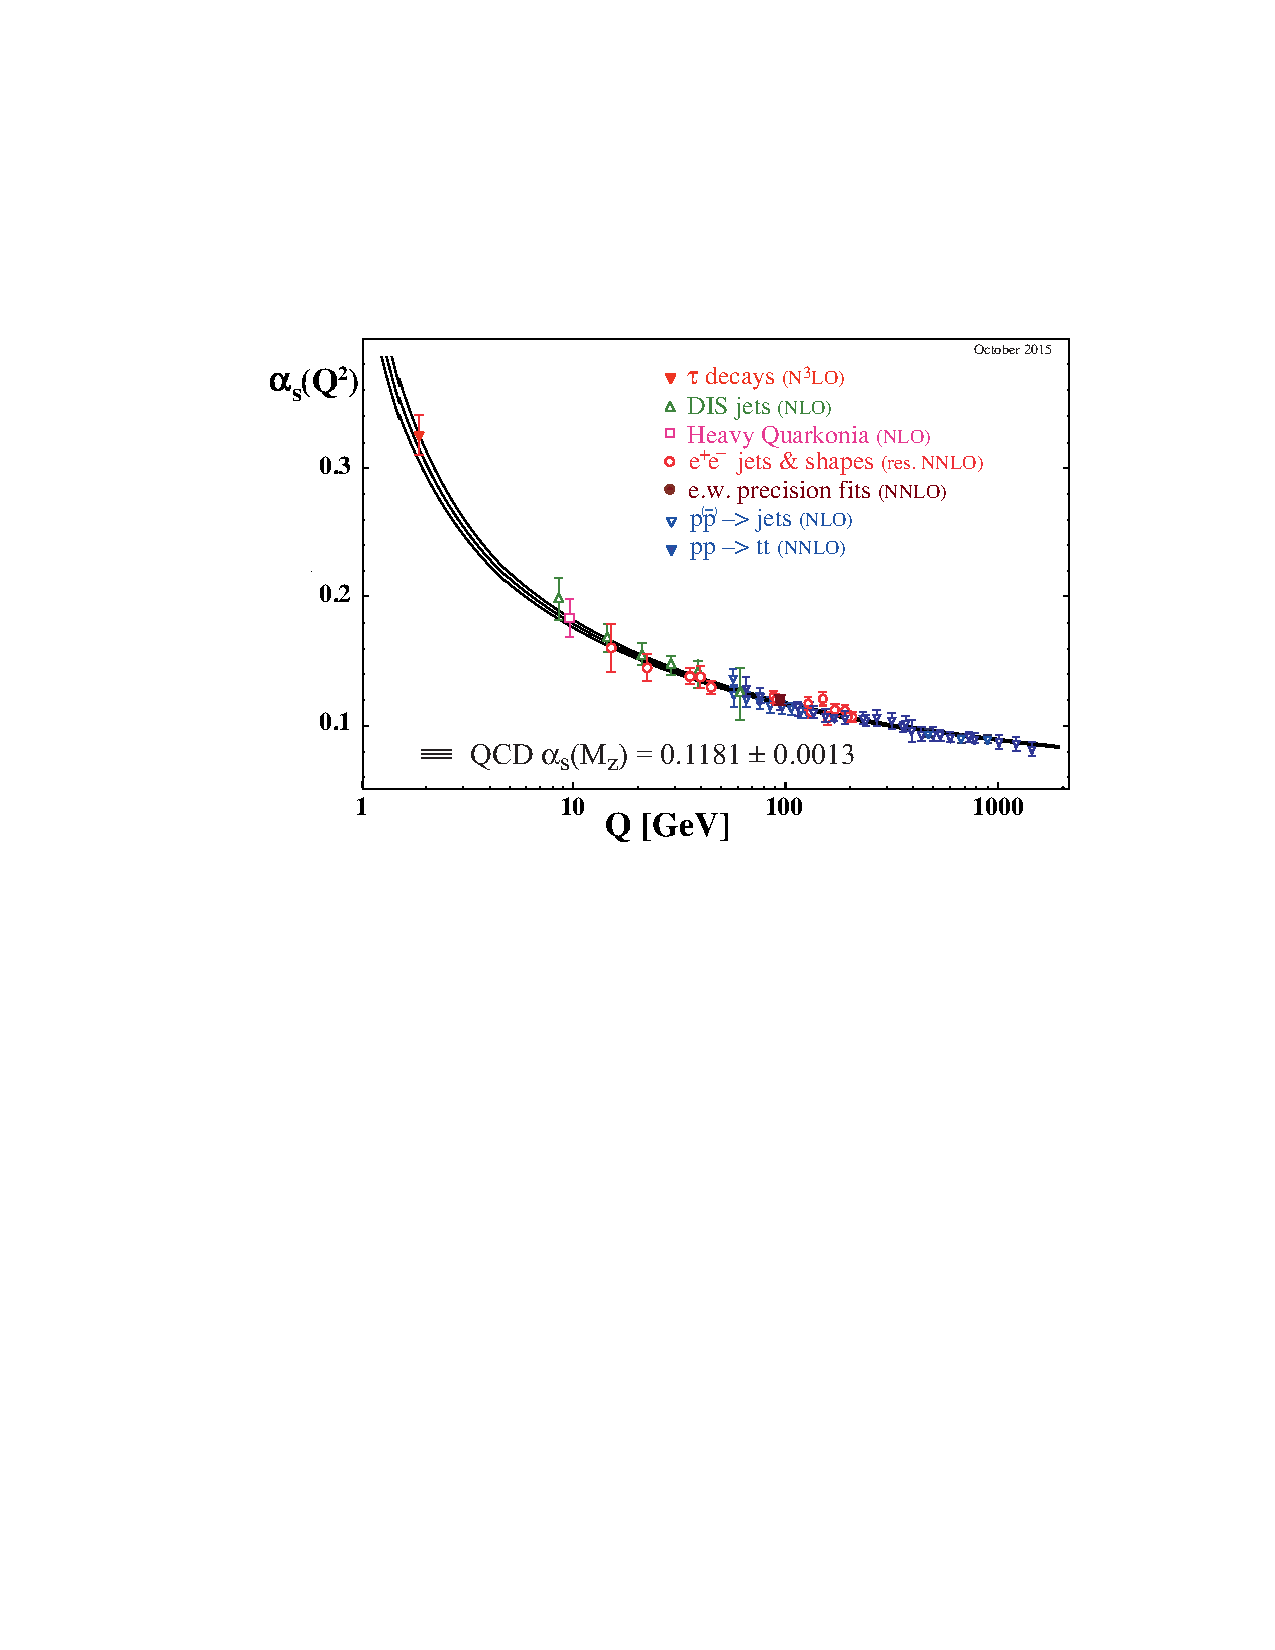
\includegraphics[width=0.7\linewidth, angle=0]{figs/Theory/qcd_running.pdf}
  \end{center}
  \caption[Summary of measurements of $\alpha_S$ as a function of the energy scale, $Q$.]
          {Summary of measurements of $\alpha_S$ as a function of the energy scale, $Q$.
            The respective degree of QCD perturbation theory used in the extraction of $\alpha_S$ is indicated in brackets
            (NLO: next-to-leading order; NNLO: next-to-next-to leading order; res. NNLO: NNLO matched with resummed next-to-leading logs; N3LO: next-to-NNLO)~\cite{theo-qcd}.}
  \label{fig:theo-qcd_running}
\end{figure}

There are three features of Figure~\ref{fig:theo-qcd_running} that should be noted.
Firstly, the size of $\alpha_S$ is generally large compared to $\alpha_{EM}$;
this means that, depending on the energy scale, the strong force is typically stronger than the EM force by one or two orders of magnitude.
Secondly, at high energies/small distances the strong force becomes relatively weak, this phenomenon is known as
\textit{`asymptotic freedom'}.
At these energy scales, perturbative expansions of QCD are possible.
Finally, at low energies/large distances the strong force is exceptionally strong.
As a result, if two interacting quarks become separated by a large distance then it becomes energetically favourable to
pair-produce $q\bar{q}$ pairs from the vacuum until a colour neutral object can be formed.
Therefore quarks are not observed in isolation, but instead quarks form colour neutral hadrons; this feature of QCD is known as \textit{`confinement'}.
At low-energy scales perturbative expansions of QCD are not possible.

\subsection{Hadronic Jet Formation}
\label{sec:theo-qcd_jets}

It is common in hadronic colliders that a high-momentum quark or gluon will be produced in the final-state
\footnote{An example of this is dijet production, as will be described in Section~\ref{sec:theo-qcd_dijet}.}.
However, due to the effect of quark confinement described above, an isolated quark or gluon will not be observed.
Instead a stream of energetic, collimated hadrons will be formed, known as a hadronic jet.
Hadronic jet formation occurs through two distinct processes; parton shower and hadronisation.

\begin{itemize}[leftmargin=*]
  
\item\textbf{Parton Shower:}

  The high-energy final-state quark or gluon will split into a $qg$ or $q\bar{q}$ pair respectively.
  The resulting quarks and gluons will also undergo splitting to form more partons,
  which in turn can split. This process continues to form the parton shower.
  Due to relativistic effects, each splitting will generally be at a small opening angle in the lab-frame
  and as such the partons will be highly collimated in the direction of the initial parton.
  The parton shower process occurs at high energy such that the value of $\alpha_S$ is small
  and thus perturbative expansions of QCD can be used to perform calculations.
  However, at each step of the splitting the energy of the partons decreases
  and thus the value of $\alpha_S$ increases.\vspace{0.5em}
  
\item\textbf{Hadronisation:}
  
  When the energy scale becomes small
  \footnote{This is generally defined as small relative to the hadronic scale, $\Lambda$, which is typically a few hundred MeV},
  $\alpha_S$ becomes large such that the dominant QCD effect is quark confinement.
  Therefore, the quarks and anti-quarks produced in the parton shower form hadrons.
  The hadrons are colour neutral objects, meaning that stable hadrons that do not interact through QCD will be formed
  \footnote{Some unstable hadrons, such as a $\Delta^{++}$, may be initially formed in the process but these will decay rapidly through the strong interaction.
    In addition, some hadrons might not be stable under the weak interaction, such as a Kaon, but the time-scale of their decays will be much larger.}.
  The hadronisation process occurs at large values of $\alpha_S$ so cannot be calculated using perturbative expansions;
  models such as the string model~\cite{theo-qcd_jet_string} and the
  cluster model~\cite{theo-qcd_jet_cluster} are used to simulate hadronisation.

\end{itemize}
  
The end result of the hadronisation process is a set of collimated stable hadrons,
known as a hadronic jet, which can be observed in an experiment.
Note that our understanding of how one goes from an initial parton to a hadronic jet is model dependant,
for example there is a choice of hadronisation model.
Hence, in experiment this dependence is removed by defining a jet in terms of observables,
such that the experimental results are model-independent and results can be reinterpreted when improved models become available
\footnote{A good explanation of why model-independent jets are desirable is found in~\cite{theo-jets_jb}}.
The details of the experimental definition of a hadronic jet is discussed in Section~\ref{sec:obj-jets}.

%\subsection{Parton shower}
%\subsection{Hadronisation}

\subsection{Dijet Production in $pp$ Collisions}
\label{sec:theo-qcd_dijet}

QCD dijet production is one of the most common processes that occurs in $pp$ colliders.
QCD dijet production occurs when the two protons interact through QCD to produce two quarks or gluons in the final state.
The free partons will then form hadronic jets through the processes described in Section~\ref{sec:theo-qcd_jets}.
Figure~\ref{fig:theo-qcd_dijet_feynman} shows the Feynman diagram of
dijet production in a $pp$ collision through the $qg \to qg$ channel.

\begin{figure}[!hbt]
\vspace{-1em}
  \begin{center}
    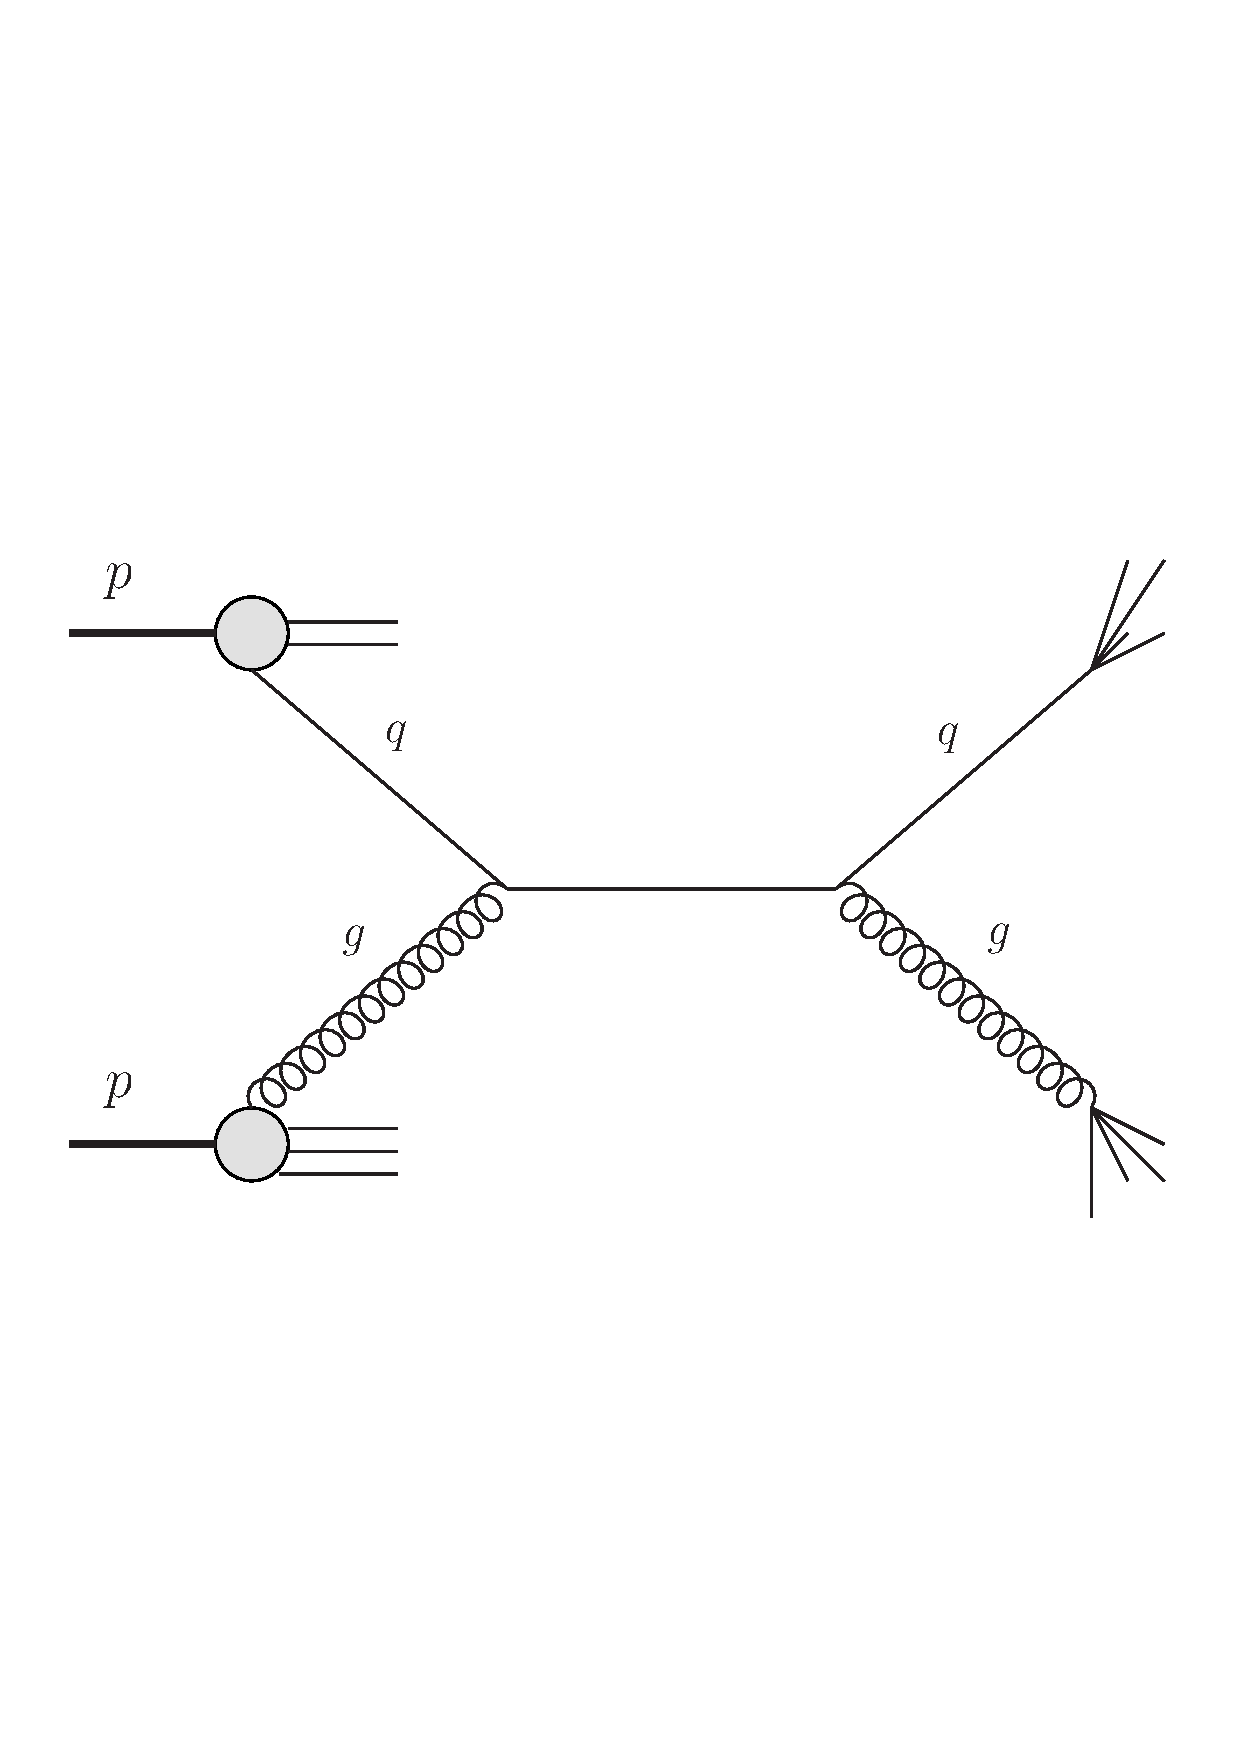
\includegraphics[width=0.65\linewidth, angle=0]{figs/Theory/qcd_dijet_feynman.pdf}
  \end{center}
%  \caption[Three feynman diagrams illustrating the parton level scatter process in dijet production at the LHC.]
  %          {Three feynman diagrams illustrating the parton level scatter process in dijet production at the LHC~\cite{theo-qcd_dijet_feynman}.}
  \vspace{-1em}
  \caption[A Feynman diagram showing dijet production in a proton--proton collision through the $qg \to qg$ channel.]
          {A Feynman diagram showing dijet production in a proton--proton collision through the $qg \to qg$ channel. Adapted from~\cite{theo-qcd_dijet_feynman}.}
          \label{fig:theo-qcd_dijet_feynman}
\vspace{-1em}
\end{figure}

The cross-section of QCD dijet production from a $pp$ collision is described by the hadronic cross-section, $\sigma_{had}$.
To calculate the hadronic cross-section, two elements are separated out in a process known as \textit{`factorisation'}.

The first element is the \textit{`parton-level cross-section'}, $\hat{\sigma}$, which is the cross-section of
two partons from the proton ($p_i$ and $p_j$) scattering to give two final state partons ($p_k$ and $p_l$).
In Figure~\ref{fig:theo-qcd_dijet_feynman}, $p_i$ and $p_j$ represent the incoming $q$ and $g$ and $p_k$ and $p_l$ represent the outgoing $q$ and $g$.
The parton-level cross section is discussed further in Section~\ref{sec:theo-qcd_dijet_xs}.
%This is effectively the central part of the Feynman diagram in Figure~\ref{fig:theo-qcd_dijet_feynman}.

The second element is the \textit{Parton Distribution Function} (PDF), $F_i(x_i)$,
which gives the number density of a specific parton, $p_i$, with momentum fraction, $x_i$, in a proton.
Momentum fraction is defined as the fraction of the proton's total momentum that the parton is carrying, $x = p_{\text{parton}}/p_{\text{proton}}$.
%The number density affects the overall cross-section, as it changes the probability that a specific parton
%can form the initial parton propagators.
This part of the interaction is indicated by the circles on the left of the Feynman diagram in Figure~\ref{fig:theo-qcd_dijet_feynman}.
Further details on PDFs is found in Section~\ref{sec:theo-qcd_pdf}.

The elements are combined to calculate $\sigma_{had}$;
\begin{equation}
%  \sigma(p_1p_2\to q/g_k q/g_l) = \int dx_1 dx_2 F_1(x_1,\mu^2_F)F_2(x_2\mu^2_F) \sigma(q/g_1,q/g_2, \alpha_s(\mu^2_R),Q^2/\mu^2_F,Q^2/\mu^2_R)
  \sigma_{had} = \sum_{i,j,k,l} \int dx_i\hspace{0.3mm} dx_j \hspace{1mm} F_i(x_i,Q^2)\hspace{1mm}F_j(x_j,Q^2)\hspace{1mm}\hat{\sigma}(p_i, p_j\to p_k p_l)
\end{equation}
where there is an integral over all possible values of momentum fractions $x_i$ and $x_j$,
a sum over all possible initial partons from the two protons labelled $i$ and $j$,
and a sum over all possible final-state partons labelled by $k$ and $l$
\footnote{The final state sums do not include top-quarks because, as will be discussed in Section~\ref{sec:theo-ttbar}, they do not form regular jets. 
  In addition, due to its heavy mass, the top-quark is heavily suppressed in the PDFs so can be ignored in the sum over initial partons.}.
$Q^2$ is the energy scale of the collision.

\noindent
With the two elements separated we can discuss each separately.

\subsubsection{Parton-level Cross-Section}
\label{sec:theo-qcd_dijet_xs}

To describe the parton-level cross-section, some useful variables must be defined.
The first is the invariant mass of the outgoing partons, $m_{kl}$, which is given in terms of the four-momentum of the two partons;
\begin{equation}
  m_{kl}^2 = (p^\mu_k + p^\mu_l)^2  
\end{equation}
\noindent
Then there are two related angular variables, $y^*$ and $\theta^*$,
defined in terms of the rapidities of the outgoing partons, $y_k$ and $y_l$;
\begin{equation}
  y^* = (\frac{y_k - y_l}{2})
\end{equation}
\begin{equation}
  cos(\theta^*) = \tanh(y^*)
\end{equation}
\noindent
Finally the Mandelstam variables are defined as, %generally used to describe a 2$\to$2 particle scatter event, 
\begin{equation}
  \hat{s} = m_{kl}^2, \hspace{3mm}  \hat{t} = -\hat{s}\hspace{1mm}(1 - \cos{\theta^*}), \hspace{3mm} \hat{u} = - \hat{s}\hspace{1mm}(1+\cos{\theta^*})
  \label{eqn:theo-mandy}
\end{equation}
The Mandelstam variables represent the square of the 4-momentum of the propagator in a 2$\to$2 particle scatter event
for an s, t or u-channel Feynman diagram respectively.

%\begin{figure}[!hbt]
%  \begin{center}
%    \feynmandiagram [horizontal=a to b] { i1 -- [fermion] a -- [gluon] i2, a -- [fermion] b,
%      f1 -- [gluon] b -- [fermion] f2,
%    };
%    \feynmandiagram [vertical=b to a] { i1 -- [fermion] a -- [gluon] i2, a -- [fermion] b,
%      f1 -- [gluon] b -- [fermion] f2,
%    };
%  \end{center}
%  \vspace{-1em}
%  \caption[]
%  {}
%  \label{fig:}
%\end{figure}

\noindent
The parton-level differential cross-section of incoming partons $i$ and $j$ scattering to give
outgoing partons $k$ and $l$ is given in terms of the variables $\theta^*$ and $m_{kl}$~\cite{theo-qcd_xs};
\begin{equation}
  \frac{d^2 \hat{\sigma}(p_i\,p_j \to p_k\,p_l)}{dm_{kl}^{2}\hspace{1mm}d\cos{\theta^*}} = \frac{ \pi \alpha_s^2}{2 \,  m_{kl}^2}
  \ \delta(x_i\,x_j\,s - m_{kl}^{2})\ \text{S}(ij \to kl) \hspace{1mm}% \frac{1}{1+\delta_{kl}}
  \label{eq:theo-qcd_dijet_xs}
\end{equation}
where $\sqrt{s}$ is the centre-of-mass energy and $\text{S}(ij \to kl)$ is the process dependant kinematics of a $ij \to kl$ parton scatter.
The $\delta(x_i x_j s - m_{kl}^{2})$ term requires that the invariant mass of the incoming partons is same as the invariant mass of the propagator.
%The $\delta_{kl}$ term prevents double-counting the case where $p_k$ and $p_l$ are identical particles.
%The $\text{S}\nobreak(ij~\to~kl)$ for each process is given in Table~\ref{tab:theo-qcd_dijet_s}.

The $\text{S}\nobreak(ij~\to~kl)$ for each process is given in Table 1 in~\cite{theo-dijet_harris}.
All but one process can occur through a t-channel diagram and therefore the 
$\text{S}\nobreak(ij~\to~kl)$ for those processes contains a $1/\,\hat{t}\,$ or $(1/\,\hat{t})^2\,$ term.
The importance of this will be discussed in Section~\ref{sec:theo-qcd-dijet_features}.

%  \begin{table}[!hbt]
%  \begin{center}
%    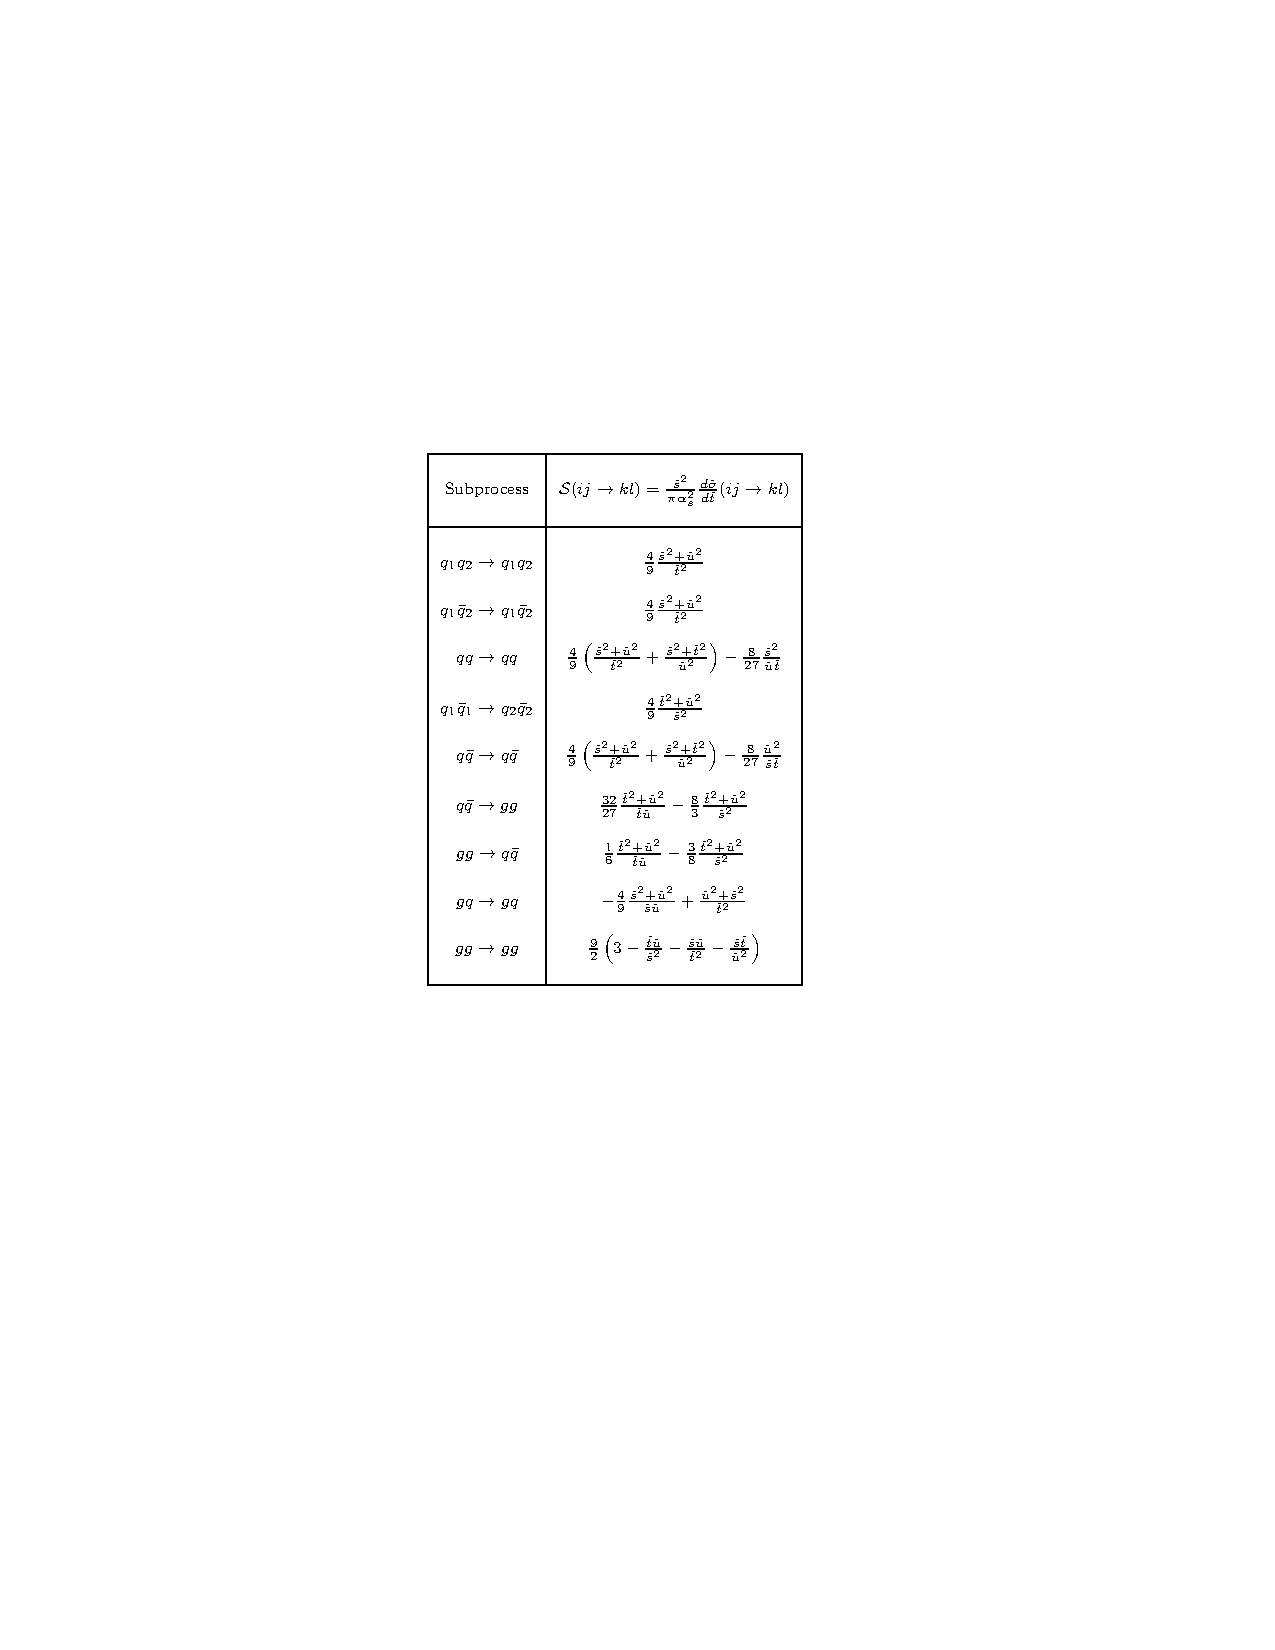
\includegraphics[width=0.5\linewidth, angle=0]{figs/Theory/qcd_dijet_stable.pdf}
%  \end{center}
%  \caption[A table showing $\text{S}(ij \to kl)$, the process dependant part of the parton cross-section, for all possible processes.]
%          {A table showing $\text{S}(ij \to kl)$, the process dependant part of the parton cross-section, for all possible processes.
%            The indices refer to quark flavour, if no indices are used then the same flavour is used for all quarks in that process. Taken from Table 1 of~\cite{theo-dijet_harris}. }
%  \label{tab:theo-qcd_dijet_s}
%\end{table}

\subsubsection{Parton Distribution Functions}
\label{sec:theo-qcd_pdf}

%A naive model of the proton contains two up-quarks and a down-quark,
%known as valence quarks, each carrying $\frac{1}{3}$ of the proton's momentum.
%However, QCD interactions within the proton mean that gluons can be emitted from the valence quarks
%and $q\bar{q}$ pairs can be produced from the emitted gluons.
The proton contains two $u$-quarks and a $d$-quark, known as valence quarks, and a sea of quarks and gluons created
through QCD interactions, such as gluons being emitted from the valence quarks and $q\bar{q}$ pairs being produced from the emitted gluons.
%The valence quarks will typically carry a lower fraction of the proton's momentum.
% typically carrying a large fraction of the proton's momentum.

Parton Distribution Functions (PDFs) give the number density of a specific parton $p_i$ in a proton $P_i$
for a given momentum fraction $x_i$ and energy scale, $Q$.
Due to the large value of $\alpha_S$ in the proton, QCD cannot be considered in perturbative expansions and as such the PDFs cannot be calculated directly.
Instead the PDFs can be measured by combining a range of experimental scattering results.
In particular, strong constraints on the PDFs come from deep inelastic scattering using $ep$ colliders, such as HERA~\cite{theo-qcd_hera};
the strong constraints are due, in part, to there only being one parton in the collision allowing direct access to the PDFs in a cross-section measurement.

%%%%%%%%%  Note Laurie %%%%%%%%%
%%%% In general one would do e- + p -> e- + jet at HERA
%%%% For sensitiviy to certain versions would could vary the analysis
%%%% For example  e- + s -> mu_e + c->D meson -> mu_e + (jet with muon).

\begin{figure}[!b]
  \begin{center}
    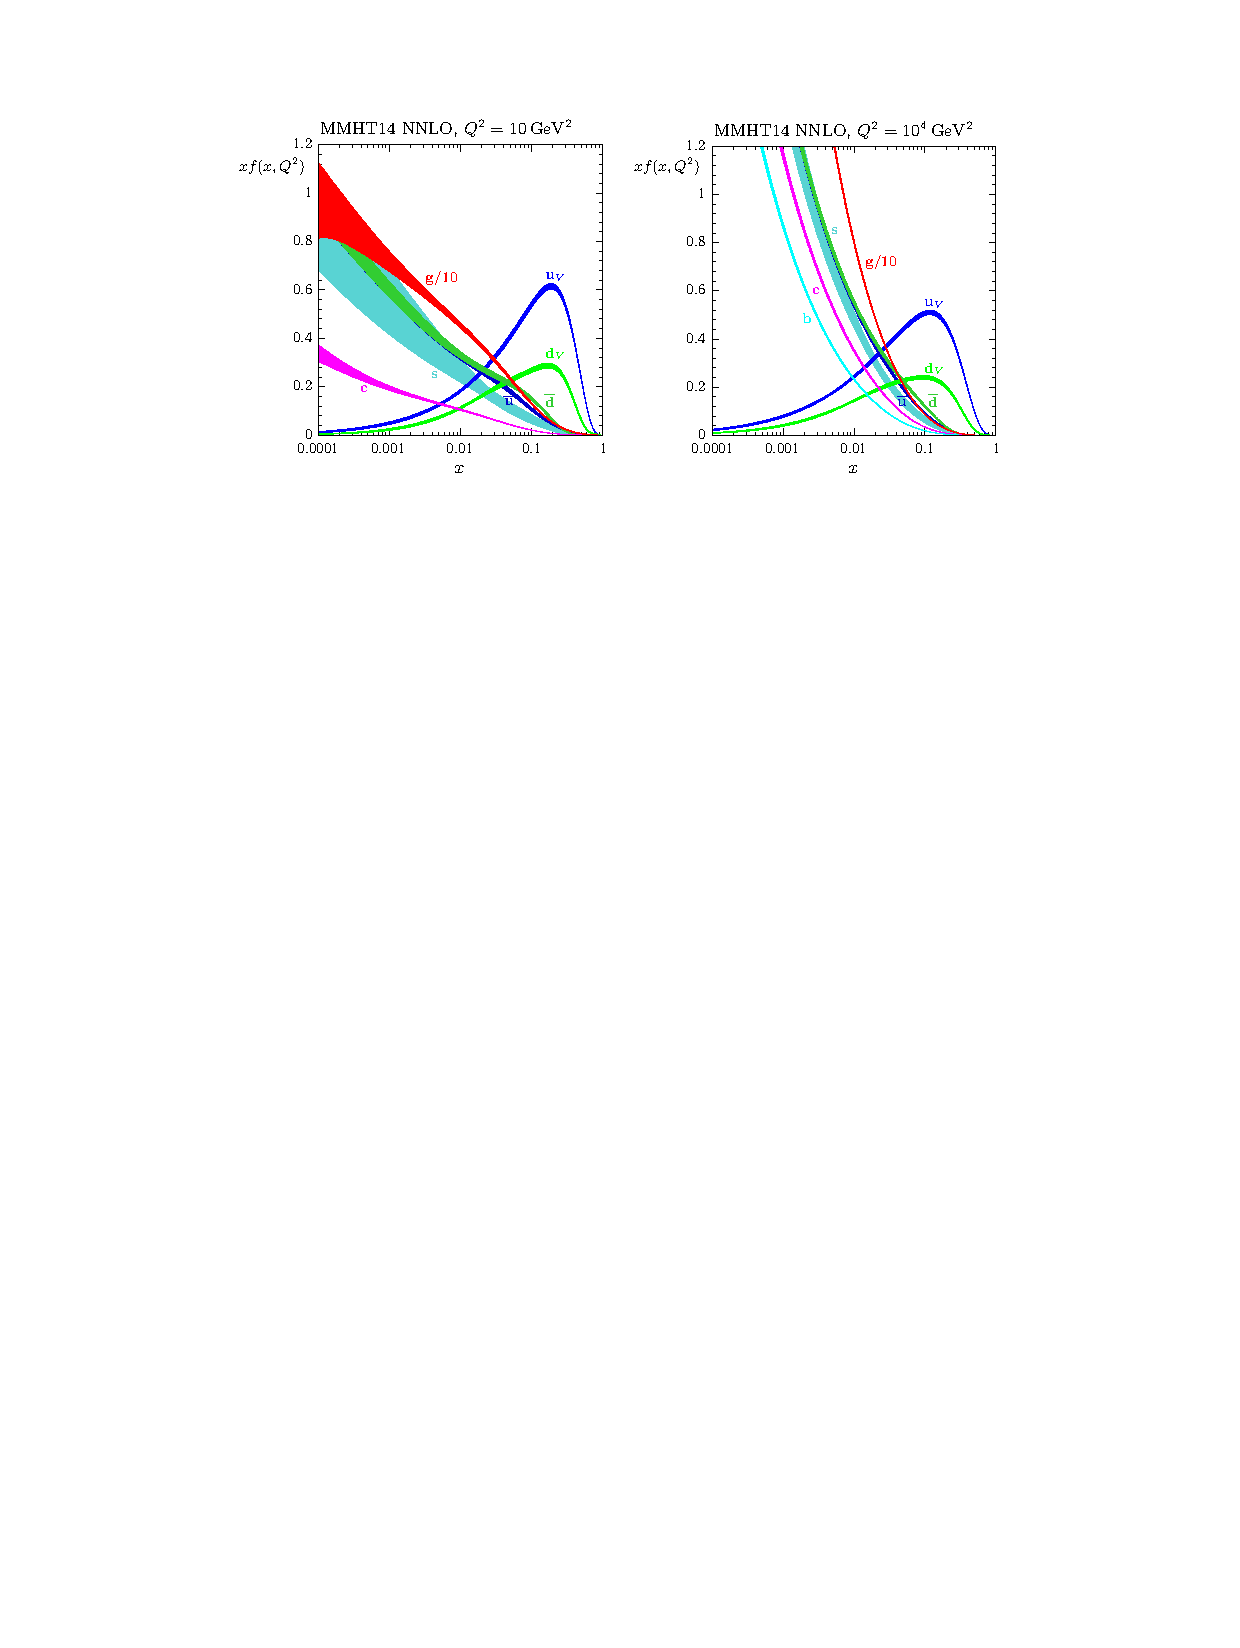
\includegraphics[width=1\linewidth, angle=0]{figs/Theory/qcd_pdf.pdf}
  \end{center}
  \caption[MMHT2014 NNLO PDFs at $Q^2$ = 10 $\text{GeV}^2$ and $Q^2$ = $10^4$ $\text{GeV}^2$, with associated 68\% confidence-level uncertainty bands.]
  {MMHT2014 NNLO PDFs at $Q^2$ = 10 $\text{GeV}^2$ and $Q^2$ = $10^4$ $\text{GeV}^2$, with associated 68\% confidence-level uncertainty bands~\cite{theo-qcd_pdf}.}
  \label{fig:theo-qcd_pdf}
\end{figure}


Figure~\ref{fig:theo-qcd_pdf} shows the $x\hspace{0.3mm}F(x,Q^2)$ for a $Q^2$ of 10 and $10^4$ $\text{GeV}^2$
from the MMHT2014 PDF set~\cite{theo-qcd_pdf}.
The various coloured lines represent the PDF for each of the different partons.
It shows that as $x$ increases the values of the PDF for the sea quarks and gluons will fall smoothly;
this is because it is energetically unfavourable to produce high momentum gluons or $q\bar{q}$ pairs.
The fall in the PDFs with respect to $x$ is particularly notable for the gluon which is the dominant contribution at large $Q^2$ and at low $x$.
The PDFs of the valence quarks, $u_v$ and $d_v$, have a peak value around $x \sim \frac{1}{3}$, and then fall off rapidly at higher $x$.
This shape is caused as at leading-order the quarks share the momentum equally, but higher-order QCD effects smear this distribution.


%If one considered the proton in the initial naive model of the proton then we find the PDFs of valence quarks as delta peaks at exactly $\frac{1}{3}$
%with amplitude of $\frac{2}{3}$ and $\frac{1}{3}$ for the $u$ and $d$ quark respectively;
%however, QCD interactions have smeared this peak to what is observed.

\subsubsection{Features of QCD Dijet Production}
\label{sec:theo-qcd-dijet_features}

From the two factorised elements discussed above,
%shown in Section~\ref{sec:theo-qcd_dijet_xs}~and~\ref{sec:theo-qcd_pdf}.t
there are four important features of the dijet hadronic cross-section
that are significant when forming the di-$b$-jet search strategy.% in Chapters~\ref{sec:evt}~and~\ref{sec:bkg}.

\begin{itemize}[leftmargin=*]
\item\textbf{Large cross-section :}\\
  The strong coupling constant $\alpha_s$ is large meaning that the dijet cross-section is large.
  Therefore QCD dijet production is the dominant background in di-$b$-jet searches.\vspace{0.5em}
  
\item\textbf{Smoothly falling with respect to $m_{kl}$ :}\\
  QCD dijet production will be smooth and monotonically decreasing
  with respect to $m_{kl}$ as a result of three factors.
  Firstly, the cross section has a $1/m_{kl}^{2}$ term.
  Secondly, as shown in Section~\ref{sec:theo-qcd_dijet_running},
  $\alpha_S$ will smoothly decrease with increasing $Q$, which in this case is correlated with $m_{kl}$.
  Finally, as $m_{kl}$ increases then the momentum fraction of the \mbox{proton, $x$,} required to create
  the dijet event will also increase.
  As shown in Figure~\ref{fig:theo-qcd_pdf}, the parton distribution functions are generally falling 
  with respect to $x$, which will lead to falling behaviour in the hadronic cross-section.
  \vspace{0.5em}
  
\item\textbf{Increased production at large values of $|y^*|$ :}\\
  A discussed in Section~\ref{sec:theo-qcd_dijet_xs}, all but one of the $\text{S}(ij \to kl)$ terms
  contains a $1/\hat{t}$ or $(1/\,\hat{t})^2\,$ contribution from t-channel Feynman diagrams.
  These terms will become large when $\hat{t} \to 0$ which, from the definition of $\hat{t}$ in Equation~\ref{eqn:theo-mandy},
  occurs when $\cos{\theta^*} \to 1$.
  This means that QCD dijet production is increased at large values of $|y^*|$.
  \vspace{0.5em}
  
\item\textbf{Preference of light-flavour quarks:}\\
  Most $ij \to kl$ processes that produce heavy flavour quarks ($c$ or $b$),
  with the exception of $q \bar{q} \to b\bar{b} \ (\text{or}\ c\bar{c})$ and $g g \to b\bar{b} \ (\text{or}\ c\bar{c})$,
  require a heavy flavour quark to be one of the initial partons.
  Figure~\ref{fig:theo-qcd_pdf} shows the heavy flavour quarks are suppressed in the PDFs relative to the other partons.
  Therefore, dijet events will be dominated by jets initiated by gluons or light-quarks ($u$, $d$ or $s$).
 
\end{itemize}

Finally, it should be noted that the above description of the QCD dijet production is not complete;
only tree-level diagrams have been considered, but there also exist higher-orders diagrams.
Related to that issue is the occurrence of initial state and final state radiation, known as ISR and FSR respectively.
ISR is when an additional parton is radiated off the incoming parton and FSR is when an additional parton is radiated off an outgoing parton.
ISR and FSR can lead to additional jets in an event, creating a multi-jet event.

In addition, there is also the Underlying Event (UE) which effectively comprises of the remnants of the proton not used in the hard-scatter.
The UE will mostly be hadronic activity and, as a result, can lead to additional jets in the event, again creating a multi-jet event.

\subsection{A Special Case: $t\bar{t}$}
\label{sec:theo-ttbar}

The top-quark is a special case when discussing the formation of jets from quarks,
due to two properties of the top-quark which are distinctive.
Firstly, the top-quark decays to a $b$-quark and a $W$ boson with a branching ratio of close to~1
because generational changing interactions involving the 3rd generation of quarks
are strongly suppressed in the the charged current weak interaction~\footnote{\ Section~\ref{sec:theo-sm_forces} contains further details of the charged current weak interaction.}.
Secondly, the top-quark is much heavier than the $b$-quark
meaning that the decay to a $b$-quark is energetically favourable.
Therefore, the top-quark decays on a shorter time-scale than parton shower processes
resulting in two separate objects; the $W$ boson and the hadronic jet containing a $b$-quark.
%\footnote{If the top-quark has a large-$p_T$ then the resulting $W$ boson and jet can merge.}.

As in dijet production, $t\bar{t}$ pairs can be pair-produced in $pp$ collisions through QCD interactions.
The two top-quarks will decay into two $W$ bosons and two jets containing $b$-quarks.
In the di-lepton decay mode of $t\bar{t}$, one $W$ boson decays into a $l^+~\nu_l$ pair and the other into a $l^{-}~\bar{\nu_l}$ pair.
A Feynman diagram showing an example of a di-lepton $t\bar{t}$ event is shown in
Figure~\ref{fig:theo-ttbar}~\footnote{\ This figure shows the $q\bar{q}$ mode of $t\bar{t}$ production. The $gg$ mode is the dominant at the LHC}.

\begin{figure}[!hbt]
  \begin{center}
    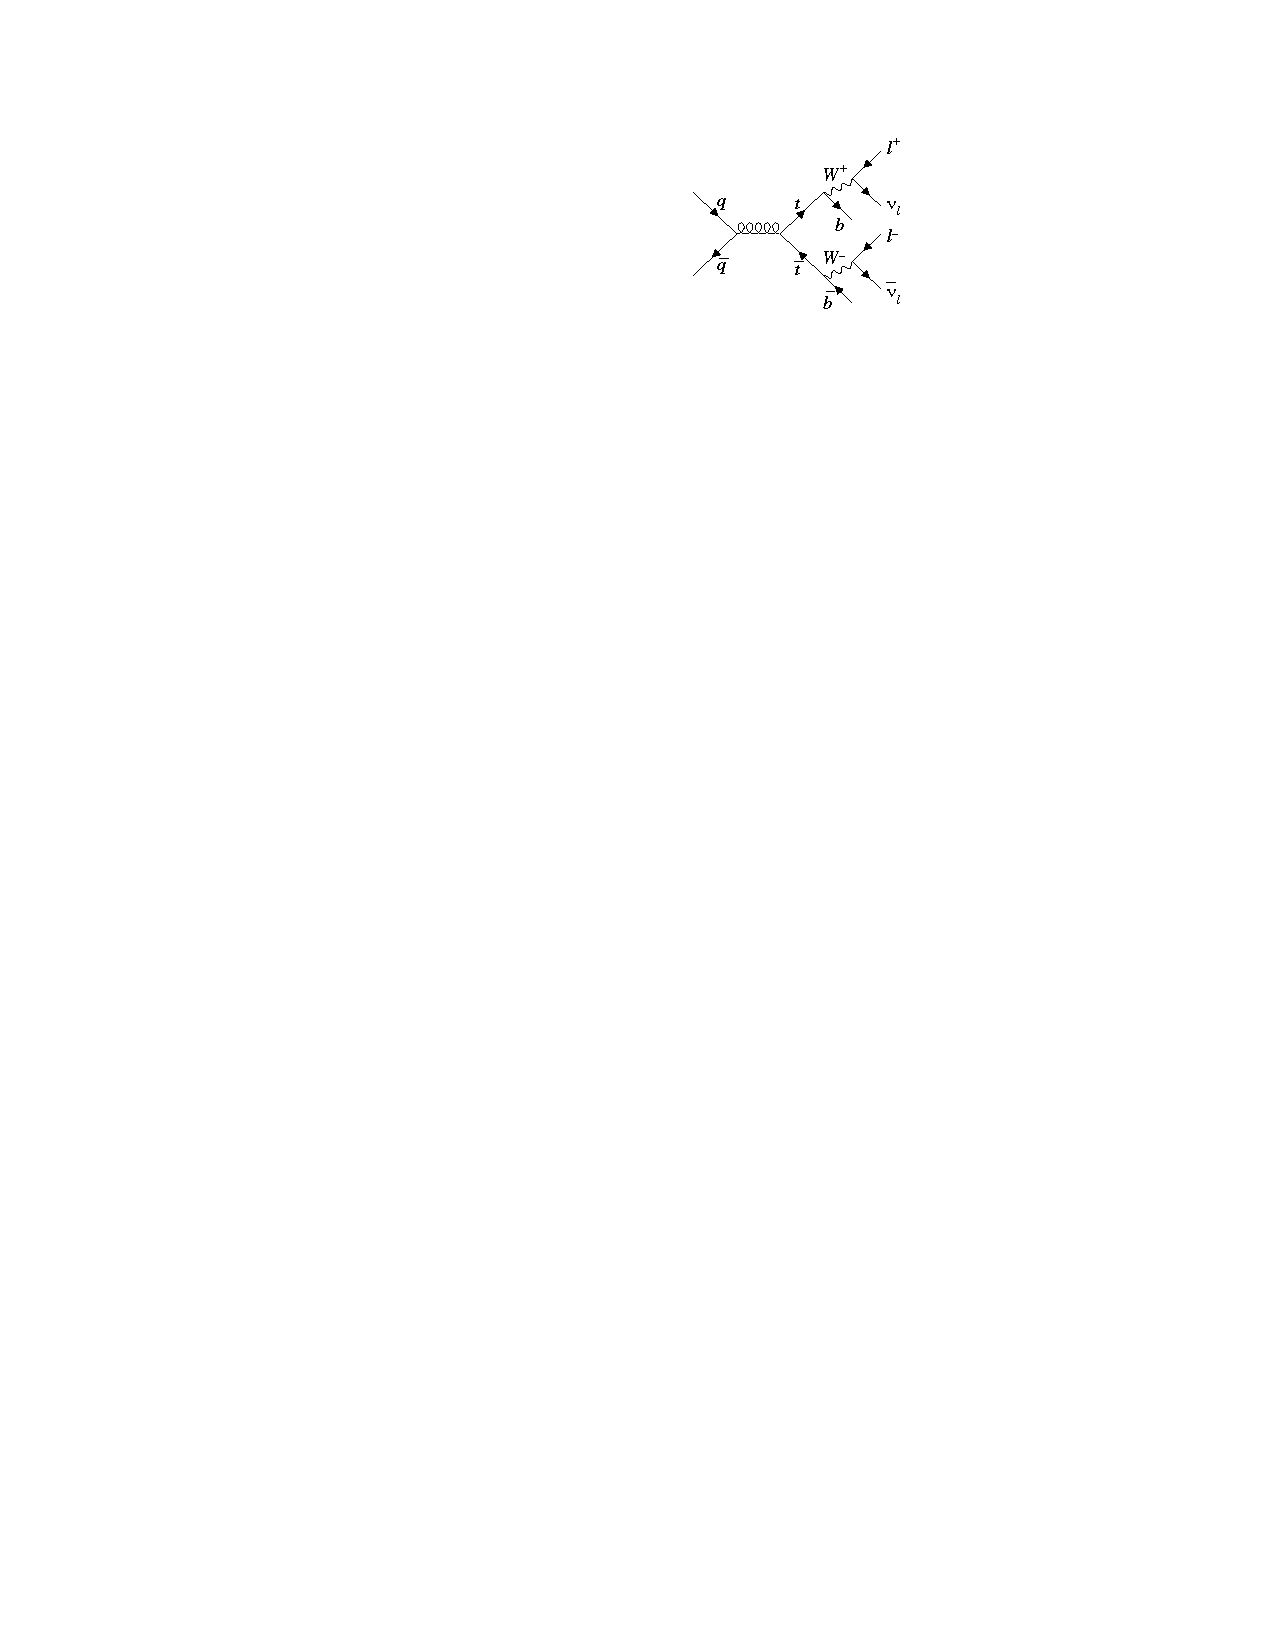
\includegraphics[width=0.6\linewidth, angle=0]{figs/Theory/ttbar.pdf}
  \end{center}
  \vspace{-1em}
  \caption[A Feynman diagram showing an example of a di-lepton $t\bar{t}$ event.]
          {A Feynman diagram showing an example of a di-lepton $t\bar{t}$ event~\cite{theo-ttbar_feyn}.}
          \label{fig:theo-ttbar}
  \vspace{-1em}
\end{figure}

Di-lepton $t\bar{t}$ events provide a distinct experimental signature.
In particular, the $e\mu$ di-lepton $t\bar{t}$ decay mode, where the leptons are an electron and a muon, is very distinct
as this can only be caused by two separate weak-decays.
%which would typically be suppressed,
%but here the large mass of the top overcomes this suppression.
In addition we have two jets formed from $b$-quarks, which can be observed.
The distinct signature of di-lepton $t\bar{t}$ events and the fact that the top-quark nearly always decays to a $b$-quark
means that this decay topology is used to obtain a pure sample of jets containing $b$-quarks,
as will be shown in Section~\ref{sec:obj-bjets_calib}~and~\ref{sec:trig-bjet_eff}.

\newpage
\section{Beyond Standard Model Physics}
\label{sec:theo-bsm}

The preceding sections of this chapter described the Standard Model and some of its successes.
%such as the prediction of the Higgs boson and the ability to describe complex phenomena such as dijet production.
However, the Standard Model is known to be an incomplete picture of the universe.
This section will present some of the key deficiencies of the Standard Model demonstrating that Beyond Standard Model (BSM) physics is required
and will discuss some proposed BSM models that motivate the analyses shown in this thesis.

\subsection{Motivations}

The motivations for BSM physics listed in this section
describe only a subset of deficiencies of the Standard Model,
with a focus on the most important missing parts and
those that motivate models searched for in this thesis.

\subsubsection{Gravity}

When listing forces in Section~\ref{sec:theo-sm_forces}, we made no reference to gravity.
This is because our description of gravity, Einstein's General Theory of Relativity,
has not been successfully merged with the Standard Model in a so-called `Quantum Theory of Gravity'.
It is a clear inadequacy of the Standard Model that there is no explanation of gravity
%partly due to the fact that gravity is hard to study at the quantum-level because
%it is so much weaker than the other forces
%(of order $10^{-39}$ compared to the strong interaction) .
% \textbf{LM Fix: Reference?}.
%There have been theoretical attempts to decribe gravity such that it is comptible with the Standard Model,
%such as the Randall-Sundrum Graviton~\cite{theo-bsm_randall},
%but so far these have not been substantiated by experimental evidence.%~\cite{trig-H4b}.

\subsubsection{Dark Matter}
\label{sec:theo_bsm_dm}

%It is remarkable that the physics that describes the largest and smallest scale known,
%Astronomy and particle physics,
%are often deeply related; the prediction of Dark Matter (DM) is a great example of this.

%Astronomers are able to make observations of distant galaxies using
%EM-waves, that allows observation of Standard Model particles  
%and are have been succesful in explaining the observed galaxies in terms of the particles of the Standard Model,
%listed in Section~\ref{sec:theo-sm_particles}.
%However, due to the large masses of astronomical objects,
%astronomers also have access to observing the action of gravity.

%Astronomers are able to make observations of distant galaxies and stars
%to study their dynamics in terms of both Standard Model processes
%and, due to the large masses of galaxies, gravitational interactions.

Astronomers have been able to make the remarkable observation that
$\sim$80\%~of the matter in universe must be so-called `dark matter'~\cite{theo-bsm_dm_peskin}.
Dark matter is not described by the Standard Model,
so is clear evidence of Beyond Standard Model physics.
It is known that dark matter interacts through gravity
and can only interact weakly, if at all, with the Standard Model,
otherwise we would have already observed it through interactions with Standard Model particles .

The evidence for dark matter comes from many separate astronomical observations:
such as studies of
galaxy rotation curves,
the cosmic microwave background
and a collision of two clusters of galaxies known as the bullet cluster,
%and galaxies using gravitataional lensing.
A wider summary of the evidence for dark matter can be found in~\cite{theo-bsm_dm_evidence}.

%\begin{figure}[!b]
%  \begin{center}
%    \captionsetup[subfigure]{aboveskip=0pt,justification=centering}
%    \subcaptionbox{Visible Spectrum}{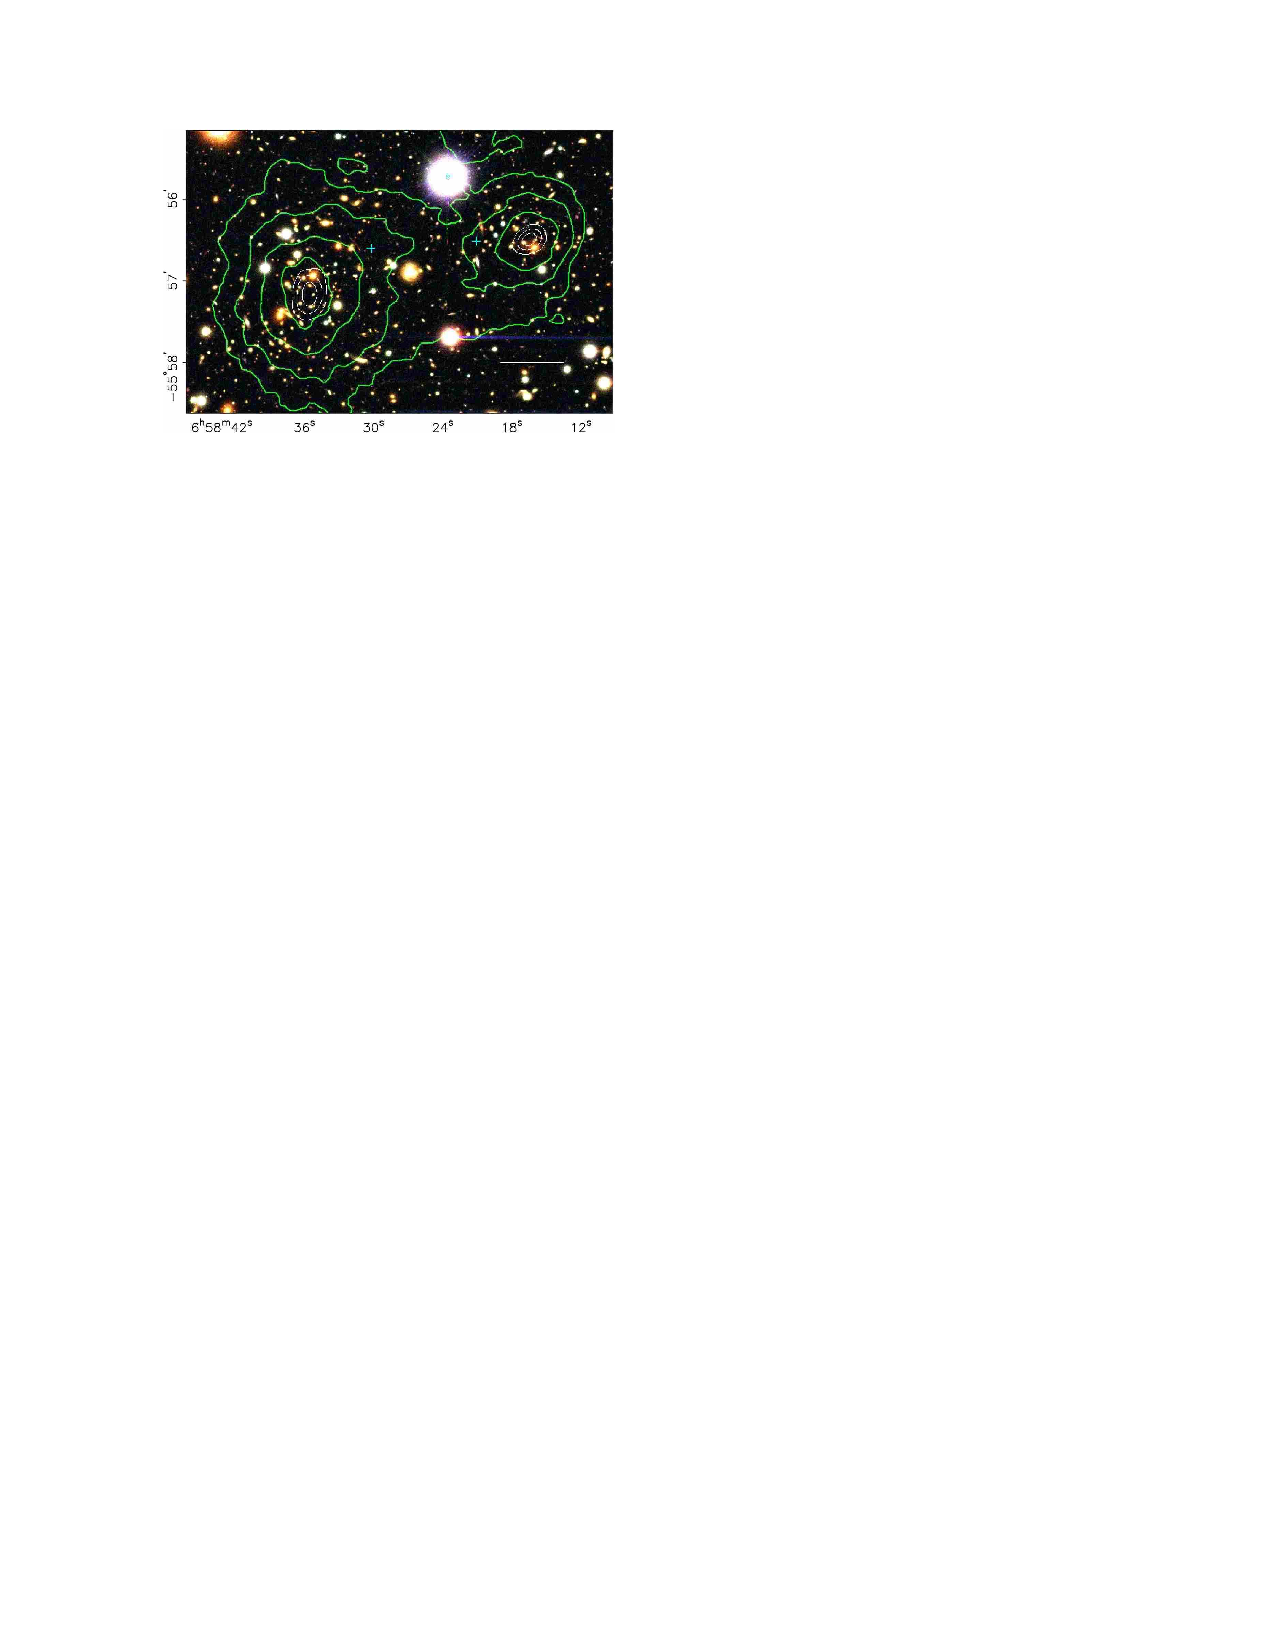
\includegraphics[width=0.48\linewidth, angle=0]{figs/Theory/bsm_gl_vis} }
%    \subcaptionbox{X-Ray Spectrum}{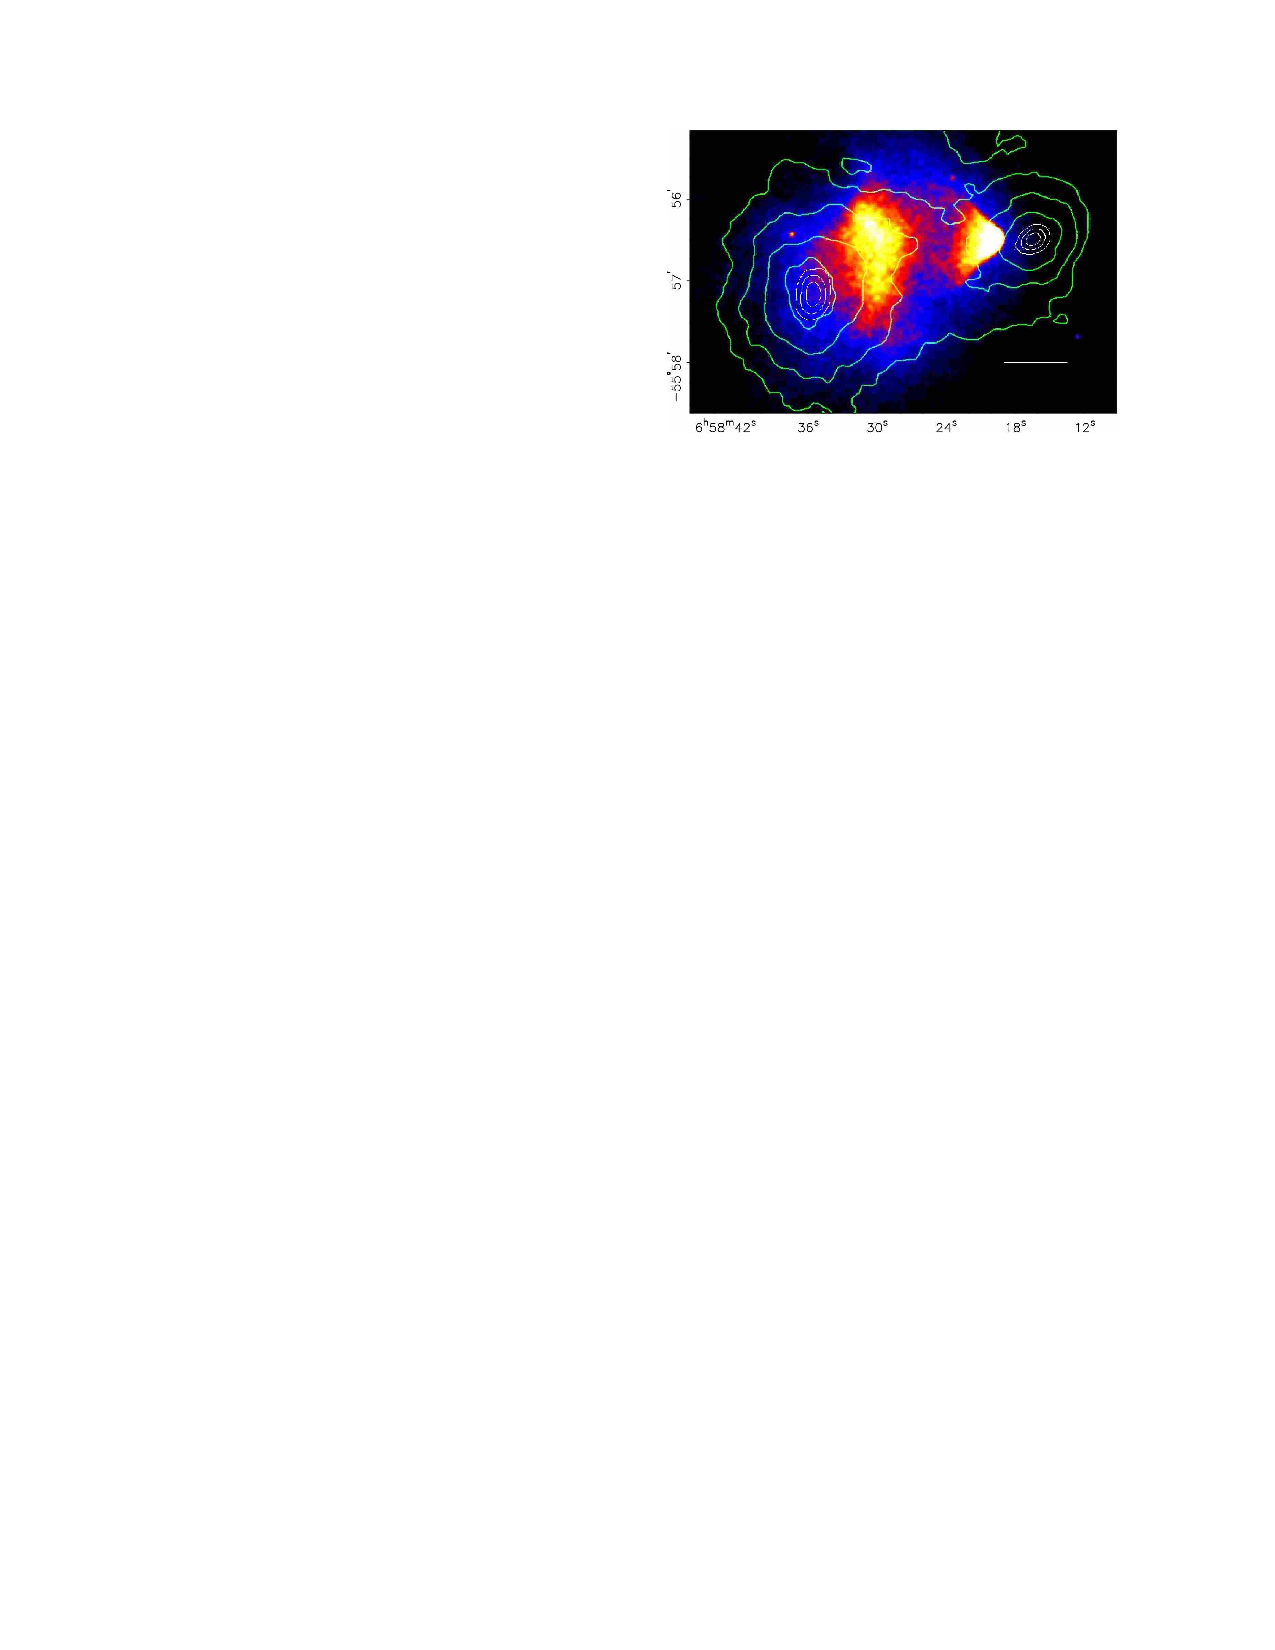
\includegraphics[width=0.48\linewidth, angle=0]{figs/Theory/bsm_gl_xray}}
%  \end{center}
%  \caption{An image of the same bullet cluster
%    (a) in the visible spectrum using the Hubble Space Telescope
%    and (b) in the X-ray spectrum using the Chandra telescope.
%    The mass density profile estimated using gravitational lensing is overlaid on both plots.}
%  \label{fig:theo-bsm_dm_gl}
%\end{figure}
%
%The cited summary provides a more rigorous explanation of the evidence than can be provided here.
%But I would like to discuss one particular bit of evidence,
%specifically measurements of bullet clusters using X-ray telescopes and gravitational lensing~\cite{theo-bsm_dm_gl}.
%Gravitational lensing occurs when the path of light from some distant astronomical source is bent by the gravitational effect of a nearer galaxy.
%Figure~\ref{fig:theo-bsm_dm_gl}(a) shows an image of a bullet cluster and the surrounding galaxies in the visible part of the light spectrum using the Hubble telescope.
%Using the gravitational lensing effect in this image one can infer the mass density profile of the bullet cluster, which is shown by the green contour lines.
%One can also observe the galaxy using an X-ray telescope,
%allowing an observation of the number density profile of Standard Model particles in a galaxy which, when hot, will emit X-ray radiation.
%Figure~\ref{fig:theo-bsm_dm_gl}(b) shows an image of the same bullet cluster in the X-ray part of the light spectrum using the Chandra telescope;
%the mass density profile estimated using the visible spectrum has again been overlaid.
%One can see that the mass density profile of the bullet cluster is inconsistent with the
%number density profile of the Standard Model particles from the X-ray telescope.
%Hence one can conclude that there must be additional Dark Matter particles in this bullet cluster
%causing the shift in the mass density profile.

Furthermore, it is believed the dark matter couples to the Standard Model.
This is required in many models of dark matter~\cite{theo-bsm_dm_feng} to explain the
observed relative abundance of dark matter particles in the universe.
As a result, this means that there may be some yet unknown mechanism that couples to both dark matter and
Standard Model particles; this mechanism is referred to as a dark matter mediator.

%The evidence for such a statement stems from the observed relative abundance of dark matter particles in the universe.
%The most common method of explaining the abundance
%, known as 'freeze-out',
%argues that in the early and hot universe dark matter and Standard Model particles
%freely interacted such that they were in thermal equilibrium.
%As the universe expanded and cooled this interaction was suppressed
%and the number density of dark matter was fixed at the value we observe today~\cite{theo-bsm_dm_feng}.
%The most common method of explaining the abundance is by postulating that
%DM and SM particles were produced in the same abundance in the Big Bang,
%and in the early hot and dense universe they could interact freely such that they are in thermal equilibrium.
%As the universe begins to cool and expand this number density will fall in equilibrium with the SM particles.
%However, at some point the universe is sufficiently cool that this interaction becomes supressed and the
%number density of dark matter is fixed at the value we observe today; this process is known as 'freeze-out'.
%As a result this means that there may be some yet unknown mechanism that couples to both dark matter and
%Standard Model particles; this mechanism is referred to as a dark matter mediator.
%%%%% Note to laurie
%% => WIMP is if mediator is weak and particle is massive
%% => WIMP miracle is that freeze-out occurs at roughly right abundance with no extra work. Great news
%% => Unfortunately WIMP is starting to become very constrained (https://arxiv.org/pdf/1507.03800.pdf)
%% => So we might need other mediator models, such as the Z'.
%\textbf{Do I need to talk about the WIMP miracle; I was going to say no as I want to talk about Z' which is not the weak force as such}

\subsubsection{Hierarchy Problem}

The Hierarchy problem~\cite{theo-hierarchy} is the fact that the energy scale of the Higgs mechanism, ($M_{H}\nobreak=\nobreak125~\text{GeV}$),
is much smaller than the energy scale of gravity,
known as the Planck scale ($M_{Planck}\nobreak\sim\nobreak10^{19}~\text{GeV}$)~\cite{obj-bjets_PDG}.
This means that the energy scale of the Standard Model is very far
from the energy scale of the next known interaction, gravity.

The Hierarchy problem leads to complications in theoretical calculations, such as that of the Higgs boson mass~\cite{theo-hierarchy}.
When calculating the Higgs boson mass, one must consider
%the bare mass of the Higgs boson from the Lagrangian in addition to
radiative contributions from additional loop diagrams,
similar to the corrections considered for a gluon propagator shown in Figure~\ref{fig:theo-qcd_gluon}. %Section~\ref{sec:theo-qcd_dijet_running}.
However, these contributions are found to be of the order $\delta m_H^2 \sim \frac{1}{16\pi^2} M_{Planck}^2$\hspace{0.2mm},
orders of magnitude larger than the observed mass of the Higgs boson.
This means that some mechanism must either cancel the contributions or reduce their size.
Whilst the free parameters of the Standard Model can be chosen such that these different contributions approximately cancel out,
such fine-tuning of the parameters is hard to believe without some underlying explanation.

Instead, there are two solutions typically proposed to stabilise the effect of the loop corrections.
Firstly, one can introduce BSM physics that has loop contributions that cancel the Standard Model contributions.
For example this occurs in theories of supersymmetry~\cite{theo-bsm_susy}.
Secondly, one can introduce some BSM physics at a new energy scale
such that the loop diagram contributions are cut off at $\delta m_H^2 \sim \frac{1}{16\pi^2} M_{BSM}^2$.
If the BSM physics is on the TeV scale then this would reduce to size of the loop corrections to the scale of the Higgs boson's mass,
giving some prior belief that new physics could be found at this energy scale.
%Both solutions could result in BSM physics around the TeV scale.

\subsubsection{Generational Structure of Quarks}
\label{sec:theo-bsm_3g}

The quarks of the Standard Model have a well ordered generational symmetry.
However the generational symmetry is not perfect;
each generation is heavier than the previous one
and within the generations quarks have different masses.
In particular, the third generation of quarks is somewhat special;
the top-quark is much heavier than the $b$-quark
and is the heaviest particle of the Standard Model.
Furthermore, as the mass of the top-quark is close to the mass of the Higgs boson,
the 3rd generation of quarks have a role symmetry breaking within the Higgs mechanism for some BSM models~\cite{theo-bsm_top}.

There is no good explanation of why there is generational structure in the Standard Model,
why the mass hierarchy is unsymmetric 
or why the third generation has one quark with such a large mass.
The generational structure could be a result of some underlying broken symmetry
which forms a part of a deeper theory of particle physics.
Any deeper theory explaining the generational structure could contain observable BSM particles,
and, given the special nature of the third generation,
the BSM particles could couple strongest with the third generation of quarks.

Unlike the case of dark matter,
the generational structure of quarks
and the special nature of the third generation is not concrete evidence of BSM physics.
But it does mean that there are motivations to be particularly interested in
searches for resonances decaying to the third generation of quarks.

\subsection{Beyond Standard Model Theories}
\label{sec:theo-bsm_models}

The previous section discussed a list of deficiencies of the Standard Model,
which makes us confident that Beyond Standard Model physics must exist.
This leads us to ask what the new theory of physics could be and
how can one obtain evidence of such a theory.

Many proposed theories of BSM physics include the addition of a new particle and,
in particular, the special nature of the third generation
\footnote{Discussed in Section~\ref{sec:theo-bsm_3g}}
means that some models of BSM predict new particles
that preferentially decay to two $b$-quarks or a $b$-quark and a gluon.
Furthermore, the Hierarchy Problem suggests that BSM physics may exist at the TeV energy-scale.
The observation of such a resonance would be evidence of BSM physics.

Two such models that predict resonances with preferential decays to $b$-quarks are discussed below.
These are used as \textit{`benchmark models'} in the analyses presented in this thesis,
where a benchmark model is a plausible signal model that is used to form and optimise a search strategy.
Furthermore the benchmark models are used to represent many models that decay to one or two $b$-quarks.

\subsubsection{$Z'$ Boson}
\label{sec:theo-bsm_zprime}

One of the most simple additions to the Standard model is that of a $U(1)'$ gauge symmetry
which would result in an additional spin-1 boson, known as the $Z'$ boson.
An additional $U(1)'$ symmetry appears in many different BSM models and is therefore a well motivated BSM extension~\cite{theo-bsm_zprime}.
The $Z'$ boson can decay to a pair of $b$-quarks, as shown in Figure~\ref{fig:theo-bsm_zprime}.
%Often theses models use the breaking of some higher gauge symmetry to give $G_{SM}~\text{x}~U'(1)^n$ gauge symmetry group,
%and thus giving additional predicting the existence of new gauge bosons in addition to the Standard Model
%\footnote{$G_{SM} = SU(3)~\text{x}~SU(2)~\text{x}~U(1)$, which is the gauge symmetry group of the Standard Model discussed in Section~\ref{sec:theo-sm}}.

\begin{figure}[!hbt]
  \begin{center}
    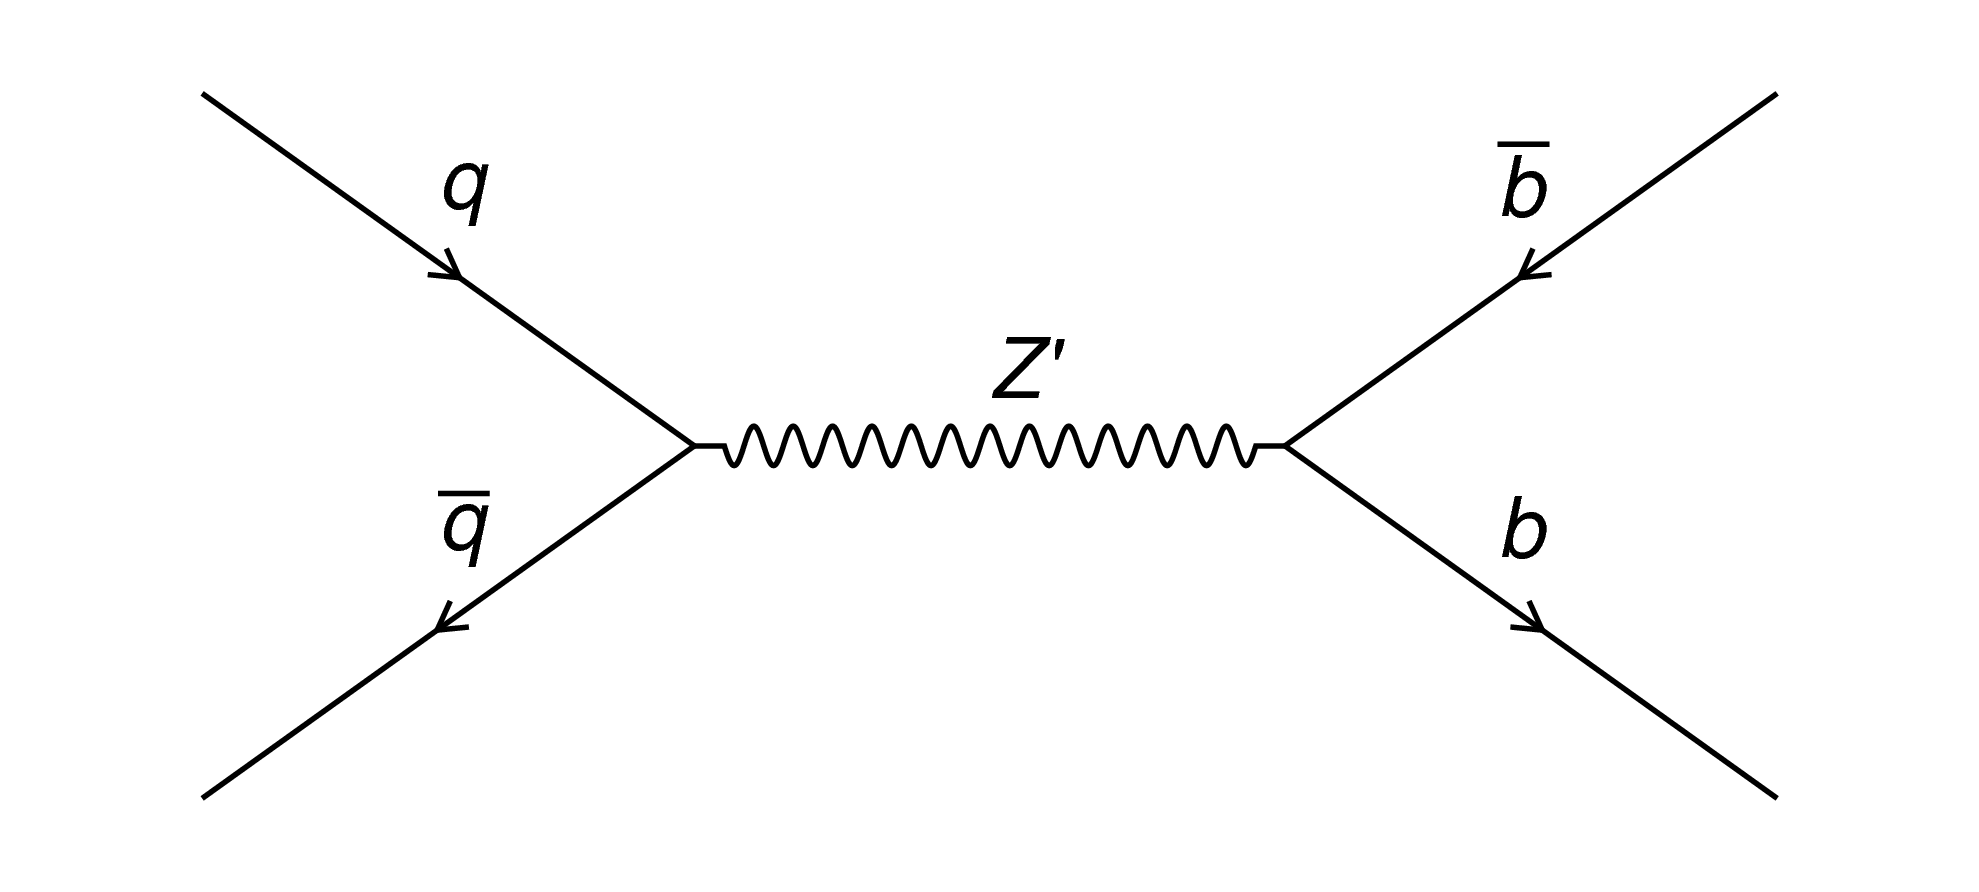
\includegraphics[width=0.7\linewidth, angle=0]{figs/Theory/bsm_zprime.png}
  \end{center}
  \caption{The leading-order Feynman diagram of the process $q\bar{q} \to Z' \to b\bar{b}$.}
  \label{fig:theo-bsm_zprime}
\end{figure}

Three different $Z'$ boson models are considered.
The first is known as the \textit{`Sequential Standard Model'} (SSM) $Z'$ in which the couplings
of the new $Z'$ boson are the same as the Standard Model.
The strongest limits on the SSM $Z'$ boson at the TeV scale are set by searching for a $Z'$ boson decaying
to lepton pairs~\cite{theo-bsm_dilep} \footnote{Because a di-lepton signature is distinct to the large QCD dijet backgrounds produced in $pp$ collisions}.

The second model is a \textit{`leptophobic'} $Z'$ boson that does not couple to the lepton sector
but has the same coupling to each of the quarks as the Standard Model~\cite{theo-bsm_zprime_leptophobic}.
This model is therefore not strongly constrained by di-lepton searches.

The final model is a \textit{`Dark Matter inspired'} (DM) $Z'$ model;
in which the DM $Z'$ boson acts as a dark matter mediator which can couple to both the dark matter sector and the Standard Model quark sector~\cite{theo_bsm-zprime_dm}.
The motivation for a dark matter mediator was discussed in Section~\ref{sec:theo_bsm_dm}.
This model introduces an additional $U(1)'$ symmetry and a Dirac fermion dark matter particle that only interacts through the new gauge group.
The resulting DM $Z'$ boson does not couple with the lepton sector
and couples with the DM fermion and the Standard Model quark sector with couplings $g_\chi$\hspace{0.1mm} and $g_{SM}$\hspace{0.1mm}, respectively.

It is worth noting in the models considered the $Z'$ boson does not preferentially decay to $b$-quarks but rather with similar branching ratio as the other quarks.
However, this can still be considered as preferential decay to $b$-quarks with respect to the dijet background
which is dominated by gluons and quarks from the first two generations, as discussed in Section~\ref{sec:theo-qcd_dijet}.
Furthermore, there exists $Z'$ models that do not couple to all generations equally~\cite{theo-bsm_zprime_3g},
such that a $Z'$ boson preferentially decaying to $b$-quarks is possible.
%For example; attempts to merge the electro-weak and strong interactions in a so-called 'Grand Unified Theory'
%often use higher symmetries, such as $SU(5)$ or $SO(10)$.

\subsubsection{Excited Third-Generation Quark}
\label{sec:theo-bsm_bstar}

To explain the generational and mass structure of the quark sector, discussed in Section~\ref{sec:theo-bsm_3g},
quark compositeness models describe quarks not as fundamental particles, but instead constructed of other fundamental particles.
One consequence of quark compositeness models is the prediction of excited quarks, $q^{*}$, which can be observed as heavy resonances.

In particular we consider an excited 3rd generation quark, the $b^{*}$ quark~\cite{theo-bsm_bstar}.
The dominant decay mode of a $b^{*}$ quark is to $bg$ with a branching ratio of 85\%
while the remaining decay modes are to $Wt$, $bZ$ and $b\gamma$ with branching ratios of 10\%, 4.5\% and 0.5\% respectively
\footnote{Using the assumptions outlined in~\cite{theo-bsm_bstar}.}.
A Feynman diagram showing the  dominant production and decay mode of a $b^*$ quark is shown in Figure~\ref{fig:theo-bsm_bstar}.

\begin{figure}[!hbt]
  \begin{center}
    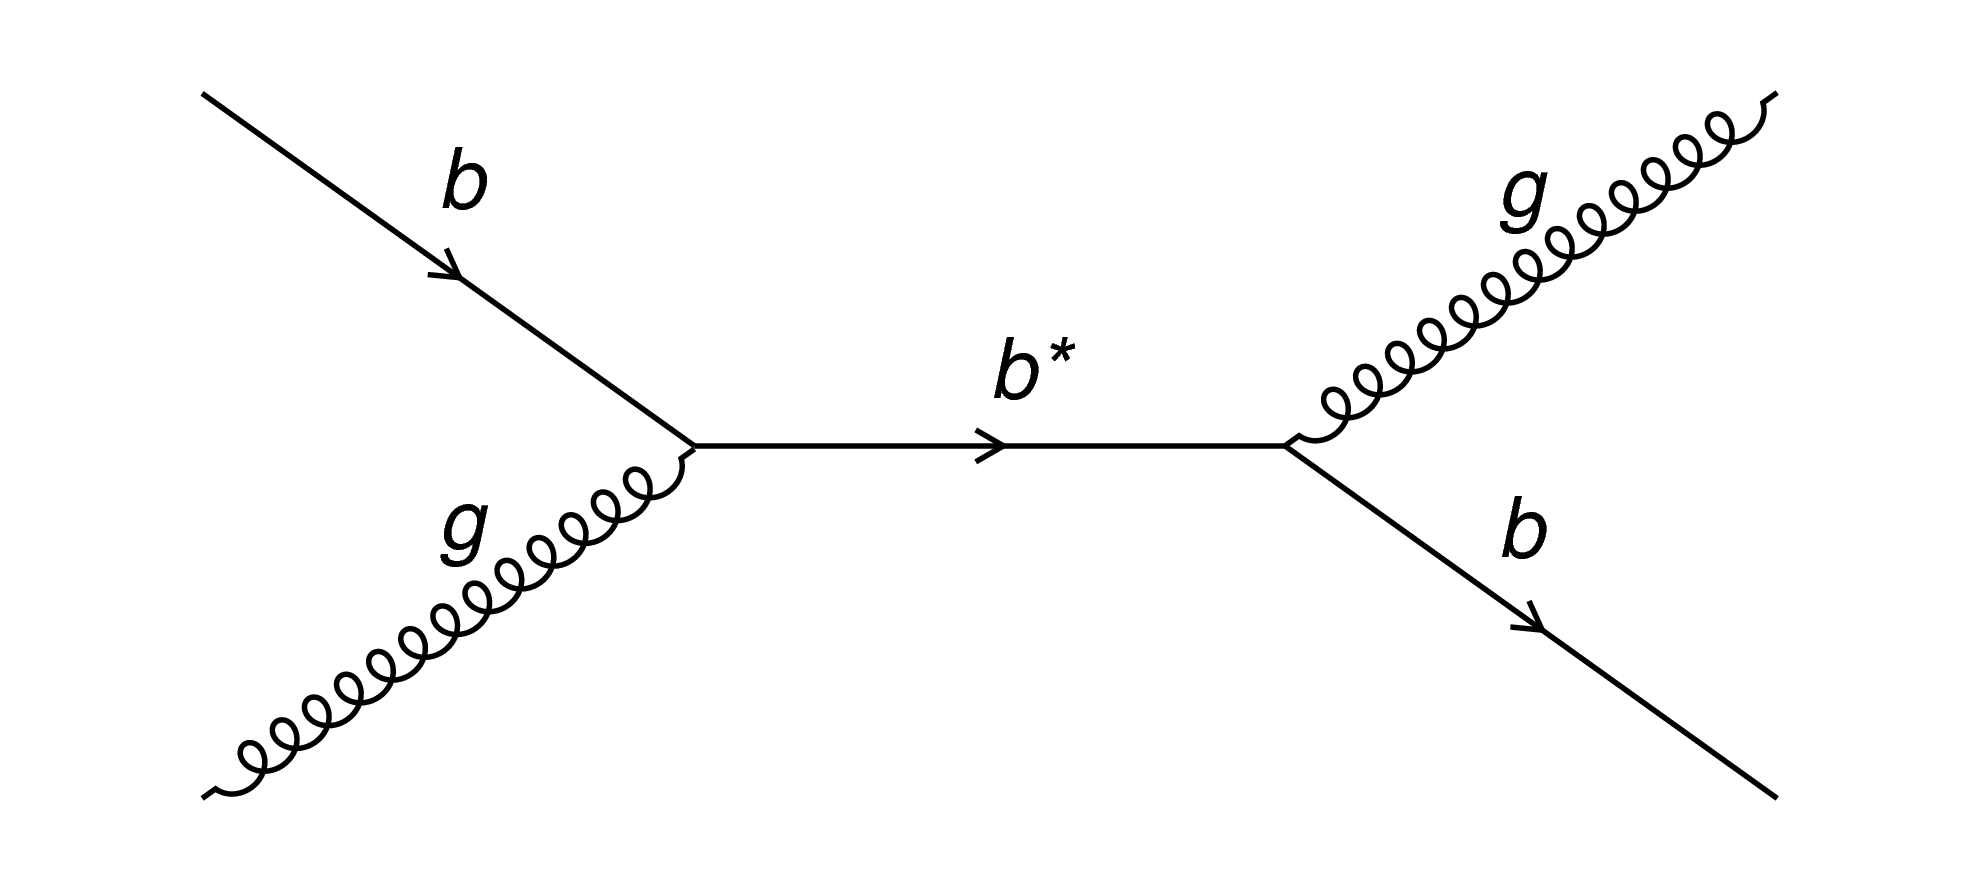
\includegraphics[width=0.7\linewidth, angle=0]{figs/Theory/bsm_bstar.png}
  \end{center}
  \caption{The leading-order Feynman diagram of the process $bg \to b^* \to bg$}
  %\caption{A Feynman diagram showing the dominant production and decay mode of a $b^{*}$ quark.}
  \label{fig:theo-bsm_bstar}
\end{figure}


\subsubsection{Model Independence}

The two benchmark models demonstrate that searching for particles decaying to one or two $b$-quarks is well motivated.
However, it is important to note that the prior belief in any specific model of BSM is small.
This is because there are many BSM theories proposed and there is little evidence to prefer one model over another.
In addition, one must also consider that the true theory may not have been anticipated, such that experiments might be able to see evidence of something truly unexpected.

%Therefore, one should construct searches for BSM to be as model independent as possible,
%rather than optimising specifically for any one model in particular.

This means that the di-$b$-jet searches should be constructed to be
sensitive to as many BSM models as possible
and allow for the unexpected gifts that nature might throw up.
